\documentclass{mproj}
\usepackage{graphicx}

\usepackage{url}
\usepackage{fancyvrb}
\usepackage[final]{pdfpages}
\usepackage{times}
\usepackage{listings}
 

% for alternative page numbering use the following package
% and see documentation for commands
%\usepackage{fancyheadings}


% other potentially useful packages
%\uspackage{amssymb,amsmath}
%\usepackage{url}
%\usepackage{fancyvrb}
%\usepackage[final]{pdfpages}

\begin{document}
\sloppy
%%%%%%%%%%%%%%%%%%%%%%%%%%%%%%%%%%%%%%%%%%%%%%%%%%%%%%%%%%%%%%%%%%%
\title{Title of project placed here}
\author{Chongbin Ren}
\date{Date of submiss}
\maketitle
%%%%%%%%%%%%%%%%%%%%%%%%%%%%%%%%%%%%%%%%%%%%%%%%%%%%%%%%%%%%%%%%%%%

%%%%%%%%%%%%%%%%%%%%%%%%%%%%%%%%%%%%%%%%%%%%%%%%%%%%%%%%%%%%%%%%%%%
\begin{abstract}
abstract goes here
\end{abstract}
%%%%%%%%%%%%%%%%%%%%%%%%%%%%%%%%%%%%%%%%%%%%%%%%%%%%%%%%%%%%%%%%%%%

%%%%%%%%%%%%%%%%%%%%%%%%%%%%%%%%%%%%%%%%%%%%%%%%%%%%%%%%%%%%%%%%%%%
\educationalconsent

%%%%%%%%%%%%%%%%%%%%%%%%%%%%%%%%%%%%%%%%%%%%%%%%%%%%%%%%%%%%%%%%%%%

\newpage
%%%%%%%%%%%%%%%%%%%%%%%%%%%%%%%%%%%%%%%%%%%%%%%%%%%%%%%%%%%%%%%%%%%
\section*{Acknowledgements}

I would like to thank the following people for their help and support throughout the project.

My supervisor, Professor Phil Trinder and Natalia Chechina, for their invaluable support and advice at all stages of doing my experiment and this dissertation. Of course, every experiment may encounter problems and failures even many upsets. However, they guide me and encourage me in different ways.

Also thanks many students who I met here and work together for the whole day and night.

I am eternally indebted to my family for supporting me and making it possible for me to complete this Master’s degree. I thank my parents who support me to have a totally different trip in a foreign country. At last, I will thank my dear girl friend who accompany me and encourage me all the time.

%%%%%%%%%%%%%%%%%%%%%%%%%%%%%%%%%%%%%%%%%%%%%%%%%%%%%%%%%%%%%%%%%%%
\tableofcontents
%%%%%%%%%%%%%%%%%%%%%%%%%%%%%%%%%%%%%%%%%%%%%%%%%%%%%%%%%%%%%%%%%%%

%%%%%%%%%%%%%%%%%%%%%%%%%%%%%%%%%%%%%%%%%%%%%%%%%%%%%%%%%%%%%%%%%%%
\chapter{Introduction}\label{intro}

\section{Context}
New industrial, personal, enterprise, and toy robots are being announced pretty much daily. There are indications that a rapid increase in the numbers of robots employed in industry is already taking place. For example, a drone is a flying robot that can be remotely controlled or fly autonomously through software-controlled flight plans in their embedded systems, working in conjunction with on board sensors and GPS[26]. The SunFounder Smart Video Car Kit for Raspberry Pi is composed of Raspberry Pi, DC-DC Step-down Voltage Module, USB camera, and  Servo Controller[27]. It can be control by an Android phone to move or take a picture. The smart car is developed based on the open-source hardware Raspberry Pi and integrates the knowledge of mechanics, electronics, and computer, thus having profound educational significance.

ROS is a software framework which can allow user to write applications and operate robotic hardware (hence Robot Operating System). ROS as it has existed for several years and has many versions. Some are older releases with long term support, making them more stable. ROS2 is a new version robot operating system but it is under heavy development. The goal of the ROS 2 project is to adapt to some changes, leveraging what is great about ROS1 and improving what is not[28].

Publishers are classes provided by the ROS library which are used to publish messages to a topic. Subscribers are classes used to receive messages from topics. Once a subscriber subscribes to a particular topic, the Master manages a connection between the publishing node and the subscribing node, so that the information is passed directly between the two processes.

This means that when you publish messages to a topic that no node subscribes too, no information is actually being communicated, since no connections have been established. When a topic has multiple subscribers, both subscribers receive the same messages since at the same time since two individual connections are setup between the publisher and each subscriber.

Messages: ROS data type used when subscribing or publishing to a topic.
Topics: Nodes can publish messages to a topic as well as subscribe to a topic to receive messages.
Master: Name service for ROS (i.e. helps nodes find each other)

\section{Object}
The aim of the research is to measure the communication performance between ROS1 and ROS2 two different robot system generation. Through sending and receiving message between multiple machines and test message latency and throughput to compare them, so that future researchers can have a understanding of two different generation ROS system communication performance.

\section{Contribution}
1. reproduce and compare different ros in different operating system
2. ros2 compare with ros1 in latency

%%%%%%%%%%%%%%%%%%%%%%%%%%%%%%%%%%%%%%%%%%%%%%%%%%%%%%%%%%%%%%%%%%%
\chapter{Background}\label{background}

\section{Robotics Overview}
Robotics is a branch of engineering that involves the conception, design, manufacture, and operation of robots[1]. Robots are machines that can be used to do jobs. Some robots can do work by themselves. Other robots must always have a person telling them what to do. Today’s robotic systems generally consist of many small autonomous systems working together to form a coherent whole[2].

This chapter aims to provide the background knowledge required to understand the results presented in this paper. Section 2.1 discusses the robotics overview and hardware in this experiment. Section 2.2 describe the operating system and robotic middleware when constructing a robotic system. Next, section 2.3 introduces network topology and communication protocol used by different robotic operating system. 

\subsection{Multi-Robot Systems}
Given the rate of technological advancements over the past decade, the adoption of robotics has become increasingly widespread. In most domains, the performance of multiple robots outperforms a single robot, both with respect to cost, efficacy and domain potential [3]. This has led to multirobot systems becoming a key area of research within the field of robotics in general [4].

Multi-robot systems can consist of many intelligent agents (each of which may be comprised of many small autonomous systems) working to solve a task that any one system may not be able to solve alone. These multirobot are distinct from a multi-agent system in which individual nodes are generally stationary, as each agent in a multi-robot system is mobile[5]. Mobile robotics has been made more possible recently by advances in battery and wireless communication technologies[6].

\subsection{Raspberry Pi}
The Raspberry Pi is a series of small single-board computers developed in the United Kingdom by the Raspberry Pi Foundation to promote teaching of basic computer science in schools and in developing countries.[7]

The Raspberry Pi is small sized like credit card, single board computer. It’s capable of doing everything that a desktop computer can do, from browsing the internet and installing applications, even playing games. It runs Linux and other available operating systems from a micro SD card. With the addition of a keyboard, mouse and micro USB power supply it can be connected to a screen monitor and used as a fully functioning desktop computer. In short, the Raspberry Pi is a small computer with relatively limited memory and performance, but it contains all needed functions.  

The first Raspberry Pi was released in 2012, since then it has been used in a vast range of projects due to its low cost, portability, programmability and both wired and wireless connectivity[8]. Several generations of Raspberry Pis have been released. The Raspberry Pi 3 and Pi Zero W (wireless) are equipped with 2.4 GHz WiFi 802.11n (150 Mbit/s) and Bluetooth 4.1 (24 Mbit/s) based on the Broadcom BCM43438 FullMAC chip with no official support for monitor mode. The Raspberry Pi 3B+ features dual-band IEEE 802.11b/g/n/ac WiFi, Bluetooth 4.2, and Gigabit Ethernet[8].

Raspberry Pi 3B+ is used in this paper. The structure picture is as follows:

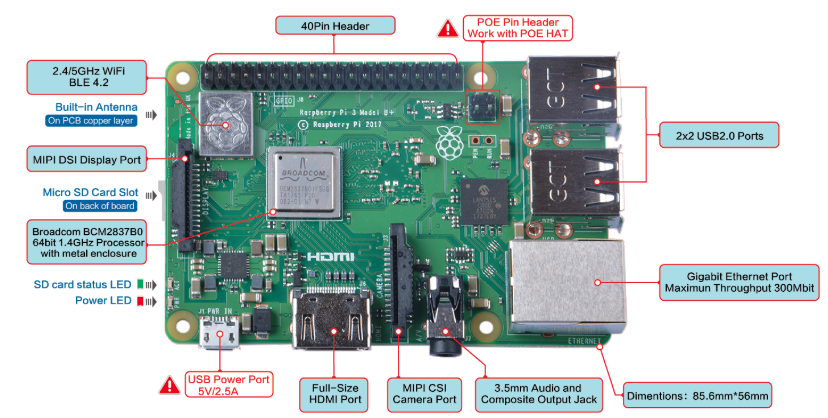
\includegraphics[width = .9\textwidth]{212.png}

\subsection{SunFounder Raspberry Pi Smart Video Car}

SunFounder is a technology company focused on Raspberry Pi and Arduino open source
community development. The Pi Car-S Robot is a smart car which work based on a Raspberry Pi.

The raspberry pi car comes with three sensor modules including ultrasonic obstacle avoidance, light follower, and line follower. The car robot has durable and shatterproof plate and new style Servo, the MAX torque of the clutch gear digital servo is up to 1.6KG[9]. It rotates from 0-180 degrees.

Python code is provided for the car, and users can also program and debug it with Dragit, a Snap-based graphical interface, by just simple dragging and dropping the code blocks for more complex functions. A user can learn the programming conveniently on how to control the car.

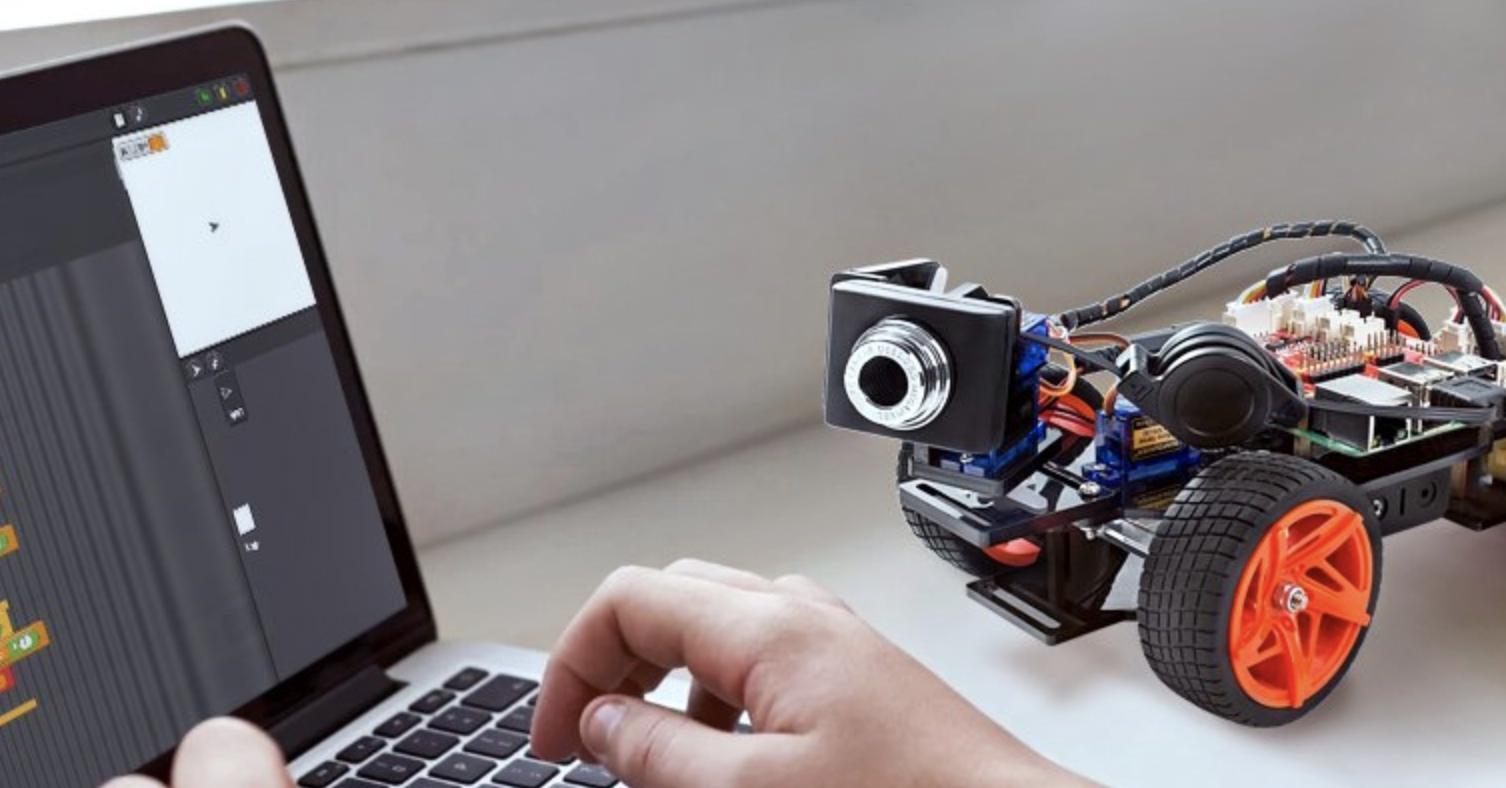
\includegraphics[width = .7\textwidth]{a.jpg}

\section{Robot Software and Operating System}
The following sections introduce the Robot software and operating system that used in this project. The version of ROS and ROS2 is under development and changes frequently these years.

\subsection{ROS}
Robot Operating System (ROS or ros) is robotics middleware (i.e. collection of software frameworks for robot software development). ROS is not an operating system. It is a set of software libraries and tools that help people build robot applications. From drivers to state-of-the-art algorithms, and with powerful developer tools and it’s all open source[11]. ROS is a software framework meant to allow people to write applications which operate robotic hardware. As its most fundamental level, it is an abstraction layer - offering hardware abstraction.  

Robotic middleware is a software infrastructure that is intended to provide convenient abstraction and communication paradigms for facilitating this multi-subsystem approach. In general, a robotics middleware would provide a common interface design so that no matter what hardware is producing the data, the results are distributed in a consistent manner[10].


Robot Operating System is mainly composed of 2 things[12]: \\
1. A core (middleware) with communication tools. \\
2. A set of plug and play libraries.

\subsection{ROS 2}
ROS2, which is a new version of ROS that is under heavy development. ROS2 is the next generation robot operating system, and is actively being developed to fully replace ROS in the near future. The goal of the ROS2 project is to adapt to previous changes, leveraging what is great about ROS and improving what is not[13]. 

A further reason to build ROS 2 is to take advantage of the opportunity to improve our user-facing APIs. A great deal of the ROS code that exists today is compatible with the client libraries as far back as the 0.4 “Mango Tango” release from February 2009. That’s great from the point of view of stability, but it also implies that we’re still living with API decisions that were made several years ago, some of which we know now to be not the best[14].

There some obvious differences between ROS and ROS2: \\
1. ROS1 is targeting Python 2, but ROS2 requires at least Python version 3.5. \\
2. Catkin make is gone: Catkin has been replaced by colcon. This new building system is in essence a universal building system for the ROS ecosystem. \\
3. ROS2 uses rclpy as Python client library which replace roscpp in ROS.

\subsection{Ubuntu}
Ubuntu is a complete Linux operating system, which is an open source Debian-based Linux distribution. Ubuntu is now the most used Linux operating system, both for desktops and servers.

Ubuntu is built on Debian's architecture and infrastructure, and comprises Linux server, desktop and discontinued phone and tablet operating system versions.[15] Ubuntu releases updated versions predictably every six months, and each release receives free support for nine months[16]. Downloading, installing, and using Ubuntu Linux doesn’t cost a penny. Installing Ubuntu does not need high-end system requirements. So it is a ideal operating system for Raspberry Pi, as the Raspberry Pi has limited memory CPU performance. 

Ubuntu is available in a number of different flavours, each coming with its own desktop environment. Ubuntu MATE takes the Ubuntu base operating system and adds the MATE Desktop. The MATE Desktop is one such implementation of a desktop environment and includes a file manager which can connect you to your local and networked files, a text editor, calculator, archive manager, image viewer, document viewer, system monitor and terminal[17]. And Ubuntu Mate offer specific downloading installing package for Raspberry Pi. This can be downloaded from the official site.

Furthermore, Ubuntu is also the recommended operating system in ROS. ROS offers more support for a few Ubuntu version. There is another operating system called Raspbian which is widely installed on Raspberry Pi. However, Raspbian is not well supported by ROS and it may occur many problems when installing ROS in Raspbian. Therefore, ubuntu is used in this experiment for Raspberry Pi as operating system.

\section{Communication on ROS vs ROS2}

\subsection{Star Network Topology}
A star topology is a topology for a Local Area Network (LAN) in which all nodes are individually connected to a central connection point, like a hub or a switch. A star takes more cable than e.g. a bus, but the benefit is that if a cable fails, only one node will be brought down[18].

All traffic emanates from the hub of the star. The central site is in control of all the nodes attached to it. The central hub is usually a fast, self contained computer and is responsible for routing all traffic to other nodes. The main advantages of a star network is that one malfunctioning node does not affect the rest of the network[19]. However this type of network can be prone to bottleneck and failure problems at the central site.

It is the most common network topology in real life, as it is easy to install, scalable and easy to troubleshoot. At the centre of the network sits the multifunctional wireless router providing the functionality of a wireless access point (WAP), a modem, a switch and a router.

Star network topology is also used in this experiment for testing message latency communicating in different devices with a center router.

The network graph is as follows:

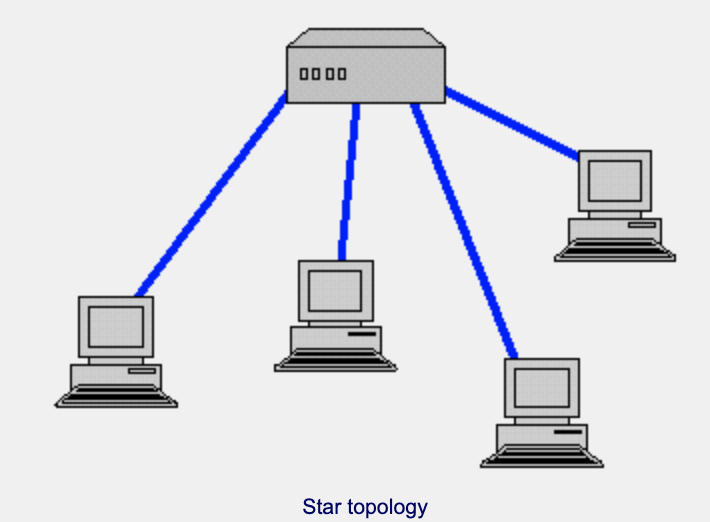
\includegraphics[width = .7\textwidth]{231.png}


\subsection{TCP and UDP in ROS}

ROS currently supports TCP/IP-based and UDP-based message transport. The TCP/IP-based transport is known as TCPROS and streams message data over persistent TCP/IP connections. TCPROS is the default transport used in ROS and is the only transport that client libraries are required to support. The UDP-based transport, which is known as UDPROS and is currently only supported in roscpp, separates messages into UDP packets. UDPROS is a low-latency, lossy transport, so is best suited for tasks like teleoperation.

ROS nodes negotiate the desired transport at runtime. For example, if a node prefers UDPROS transport but the other Node does not support it, it can fallback on TCPROS transport[20]. This negotiation model enables new transports to be added over time as compelling use cases arise.

TCPROS is a transport layer for ROS Messages and Services. It uses standard TCP/IP sockets for transporting message data. Inbound connections are received via a TCP Server Socket with a header containing message data type and routing information[21]. 

Therefore, in the experiment, ROS use TCPROS to communicate between different machines by default.
The TCPROS communication structure is as follows:

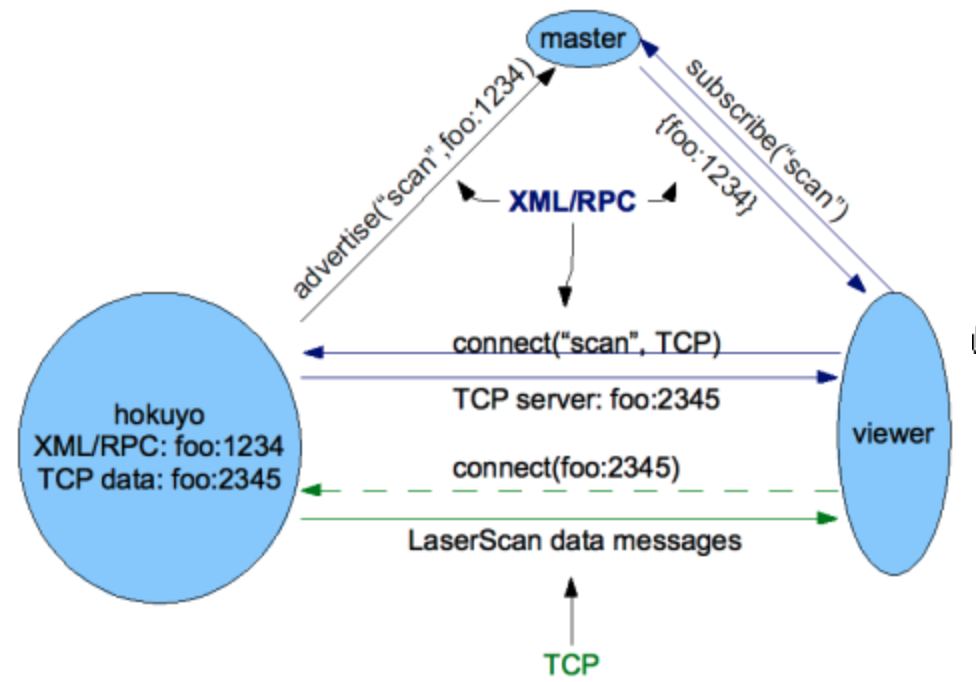
\includegraphics[width = .7\textwidth]{d.png}

\subsection{Data Distribution Service (DDS) on ROS2}
When exploring options for the next generation communication system of ROS, the initial options were to either improve the ROS 1 transport or build a new middleware using component libraries such as ZeroMQ, Protocol Buffers, and zeroconf (Bonjour/Avahi)[22]. However, in addition to those options, during the research, one middleware that stood out was DDS.

The benefit of using DDS, is that there is much less code to maintain and the behavior and exact specifications of the middleware have already been distilled into documentation. In addition to system-level documentation, DDS also has recommended use cases and a software API. With this concrete specification, third parties can review, audit, and implement the middleware with varying degrees of interoperability. This is something that ROS has never had, besides a few basic descriptions in a wiki and a reference implementation[23].

ROS2 using DDS as message transport service. DDS provides a publish-subscribe transport which is very similar to ROS’s publish-subscribe transport. It allows any two DDS programs to communicate without the need for a tool like the ROS master[24]. This makes the system more fault tolerant and flexible.

The default implementation of DDS is over UDP,  DDS implementations use (UDP) broadcast traffic for peer discovery. By default, when sending message, the ROS2 communication will broadcast to the local subnet (ie: all IPs in the same range).

%%%%%%%%%%%%%%%%%%%%%%%%%%%%%%%%%%%%%%%%%%%%%%%%%%%%%%%%%%%%%%%%%%%
\chapter{Installation and configuration}

\section{Ubuntu and ROS system installation}

\subsection{Ubuntu installation}
1. Download the latest version image of Ubuntu Bionic (64-bits) for Raspberry Pi from official website.

2. Write the image to Raspberry Pi 3B+ by using SD card.

3. Run it with screen and configure all necessary dependency and install "openssh" server for remote control.
 
\textbf{Issues and Solution} 

1. Other operating system like Raspbian 10(buster) is not well supported by ROS system. There are some outdated dependencies which is needed in installing ROS. Therefore, there are many bugs and manually installation steps to solve when user want to install ROS in Raspbian operating system. Then the Ubuntu is recommend operating system as official website said.

2. Find the 64-bits version operating system because ROS2 only can run on 64-bits operating system.

\subsection{ROS1 Installation}

1. Follow the step details at first appendix A1 ROS1.

2. Configure Ubuntu repositories to allow "restricted," "universe," and "multiverse."

3. After installation, use \textit{roscore} to test whether ROS system exist.

\subsection{ROS2 Installation}

1. Installing ROS2 via Debian Packages.

2. Follow the step details at first appendix A2 ROS2. 

3. Using \textit{ros2 run XXpackage XXfile} to test whether ROS2 can run successfully.


\section{Router network configuration}
1. Each Raspberry Pi should connect to the same LAN.

2. Assign static IP address to each Raspberry Pi for ssh remote control and management.

3. Using one computer to join this LAN for controlling the all Raspberry Pi.

4. Remote control other Raspberry Pi by ssh using \textit{ssh {hostname}@{ip address}} with password.


\section{Communication between different ROS hosts}
\textbf{Change the host file} 

Each host configuration file can be modify by \textit{sudo vim /etc/hosts}. Add ip address and hostname in \textit{/etc/hosts} file for Raspberry Pi. Each ip address respond to one hostname which you give.
Example hosts file is in the Appendix.

\textbf{Running Talker and Listener}

Enter ROS system in every Ubuntu system and ssh to com1. Then ping com1 and com2. If ping successfully meaning the network is fine, otherwise check the router and network problem.

The host name and ip address is respond to each Raspberry Pi, but the Master URI should be identical. Create a  \textit{.sh} file to export environment paths. See the appendix

Configure the file and execute this file in every Raspberry Pi host. Then run the talker and listener python file seperately in different hosts to check if listener can receive messages from talker.

\textbf{Issues and Solution}

Make sure setting the ROS hostname and IP address correctly and must explicitly set it. Otherwise the listener cannot receive talker because the host cannot find it in the network. The Talker will send messages continuously but listener can not receive these messages.

Check the hostname and ip address setting can use:
\begin{verbatim}
echo $ROS_HOSTNAME
echo $ROS_IP
\end{verbatim}

%%%%%%%%%%%%%%%%%%%%%%%%%%%%%%%%%%%%%%%%%%%%%%%%%%%%%%%%%%%%%%%%%%%
\chapter{Experiment and Analysis}

\section{Experiment 1: Comparing different ROS1 version  with previous experiment}
\textbf{Objective} \\
This experiment investigates the performance in different frequency of message passing by using Wi-Fi network connection in a router.  This experiment was executed by Issac in the previous and my aim is execute this experiment to compare it with the previous one[25].

\textbf{Rationale} \\
In order to acquire a detailed understanding of the performance characteristics of ROS’ communication channels, this experiment use two ROS hosts to commnunicate with each other and get the message latency results in different message frequency. I reproduced Issac's experiment to see what is the difference between my experiment and the previous one then analyze the reason to cause these differences.

\textbf{Procedure} \\
1. Start one master node on one host and send different frequency message to a echoer node on another host by using Wifi network. \\
2. Run the code which send timestamped messages from the sender host to the echoer host. Then the echoer host receive message and send it back to master host. \\
3. The master node will receive the message and then record message id and time in sending and receving into a file.  \\
4. Message frequency is from 200 to 2000Hz (200,400,600...2000)which is same with Issac experiment. \\
5. Every frequency will be recorded 3 times with a range of message frequencies to obtain averaged results for each message frequency. \\
6. Running this experiment in different ROS1 version and operating system.

\textbf{Hardware Configuration} \\
4 Raspberry Pi 3B+ \\
TP-Link 150M Router

\textbf{Software Configuration} \\
Ubuntu 18.04 Bionic (64-bit)\\
ROS Melodic (Latest, Released May, 2018) \\
Ubuntu 16.04 Xenial (32-bit) \\
ROS Kinetic Kame (Released May, 2016)

\textbf{Hypothesis} \\
1. The message latency should be like the previous experiment results. \\
2. Different message frequency may perform different latency. For example, lower message frequency can have lower message latency. \\
\textbf{Results} \\
The previous experiment from Issac is Figure 4.1. I only plot six different frequency instead of Issac 10 frequency because it may make the graph more clear to check out. The Figure 4.2 is message latency from ROS kinetic on Ubuntu Xenial and the figure 4.3 is ROS Melodic on Ubuntu Bionic.


\begin{figure}[h!]
\centering
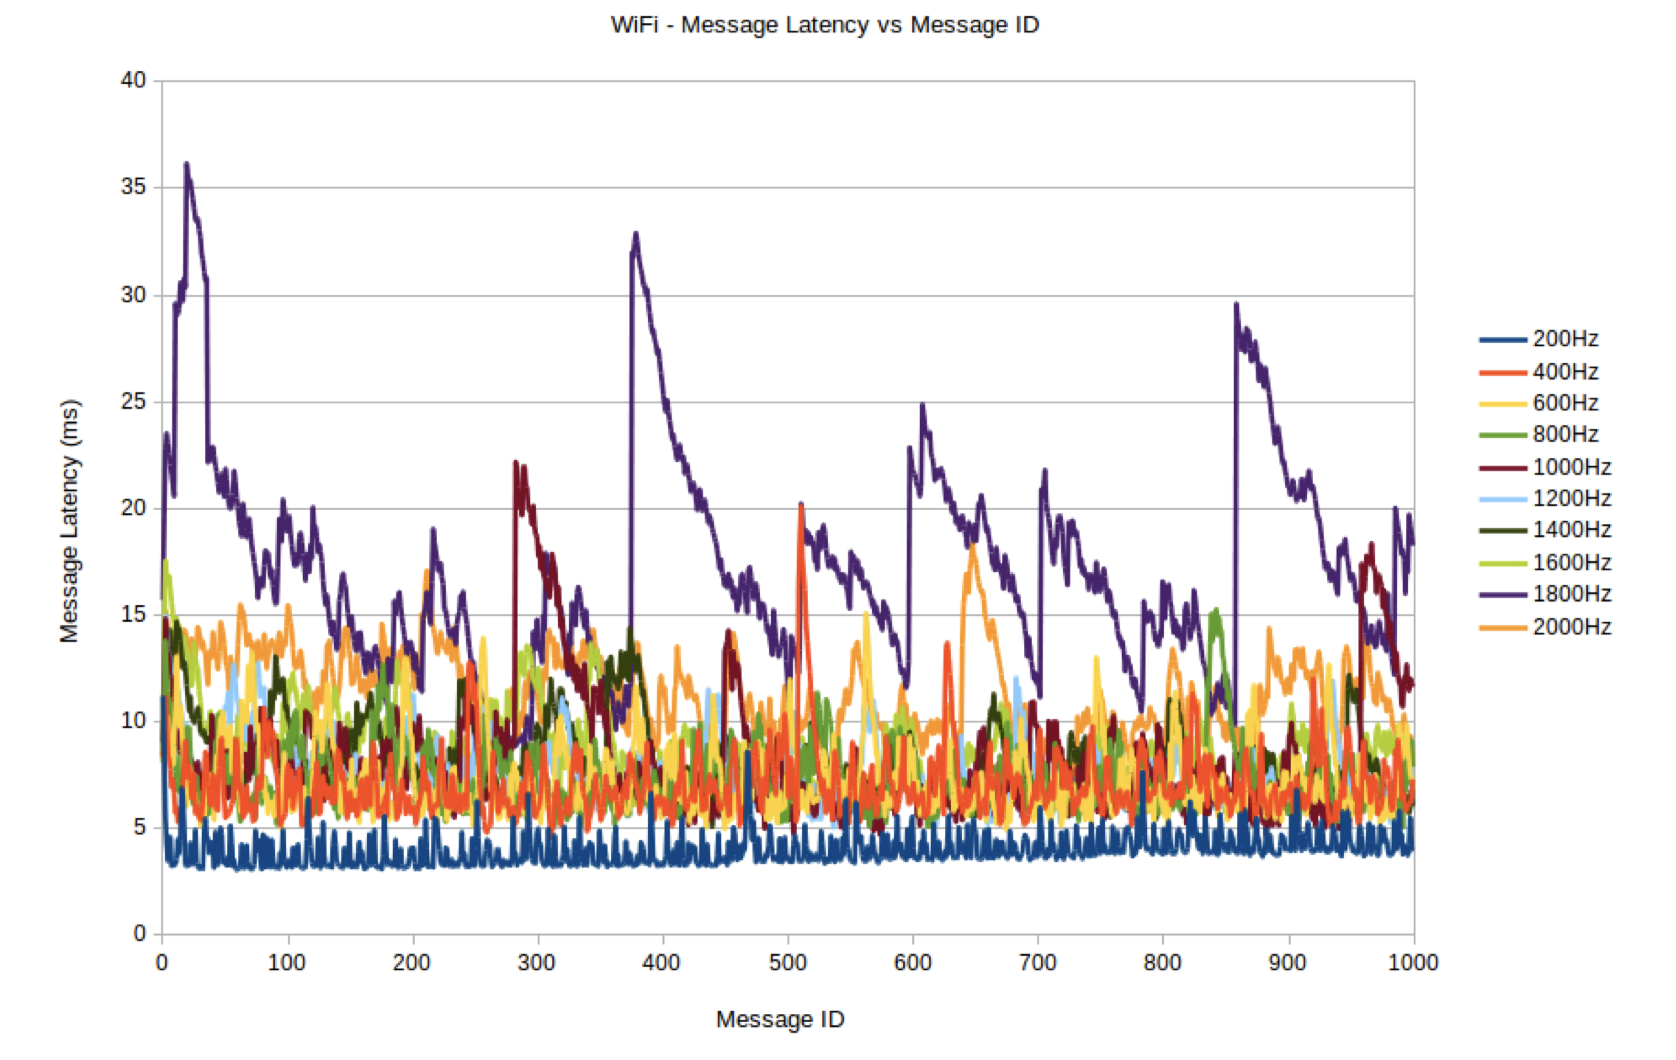
\includegraphics[width = 1\textwidth]{ex1_issac.png}
\caption{Message latency for all frequency in Issac experiment}
\end{figure}

\begin{figure}[h!]
\centering
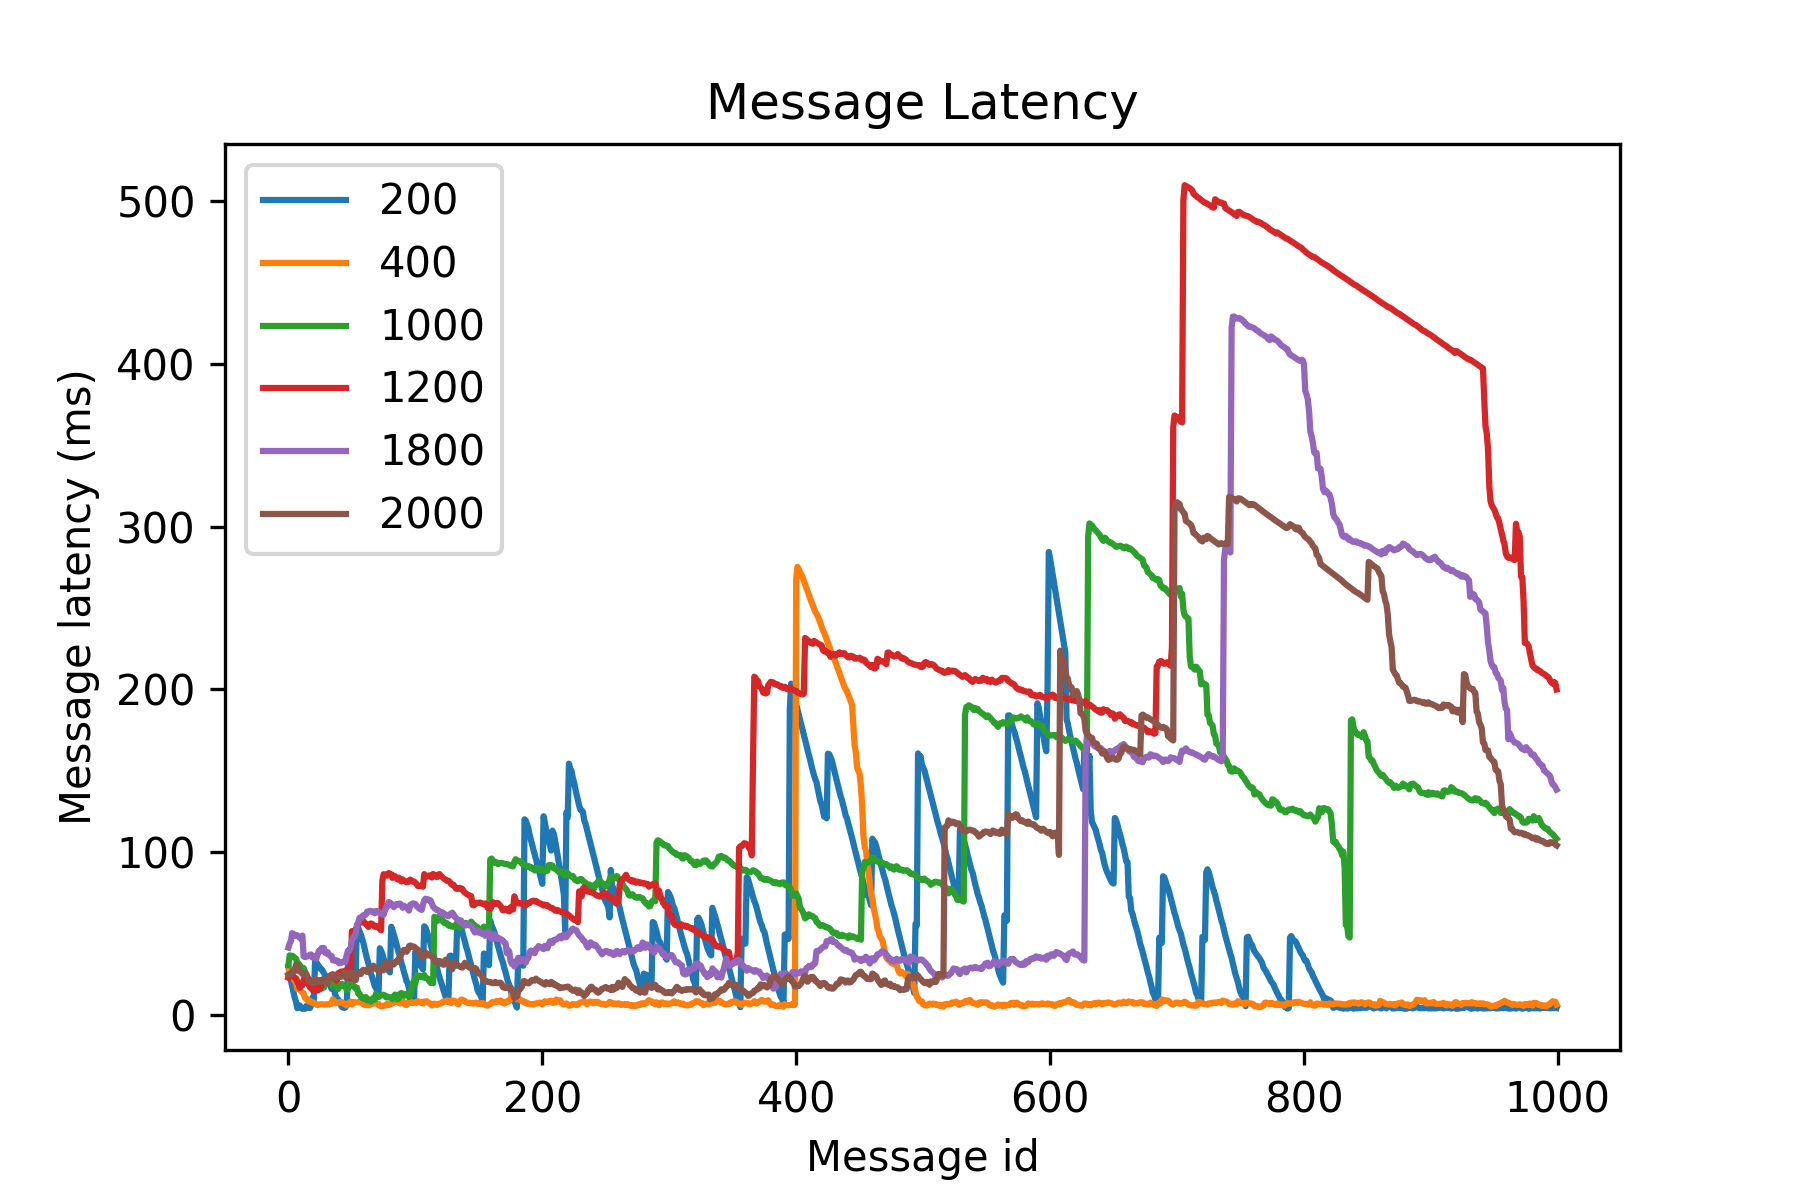
\includegraphics[width = 1\textwidth]{ex1_res1.png}
\caption{Message latency for ROS kinetic on Ubuntu Xenial 32-bit}
\end{figure}
\begin{figure}[h!]
\centering
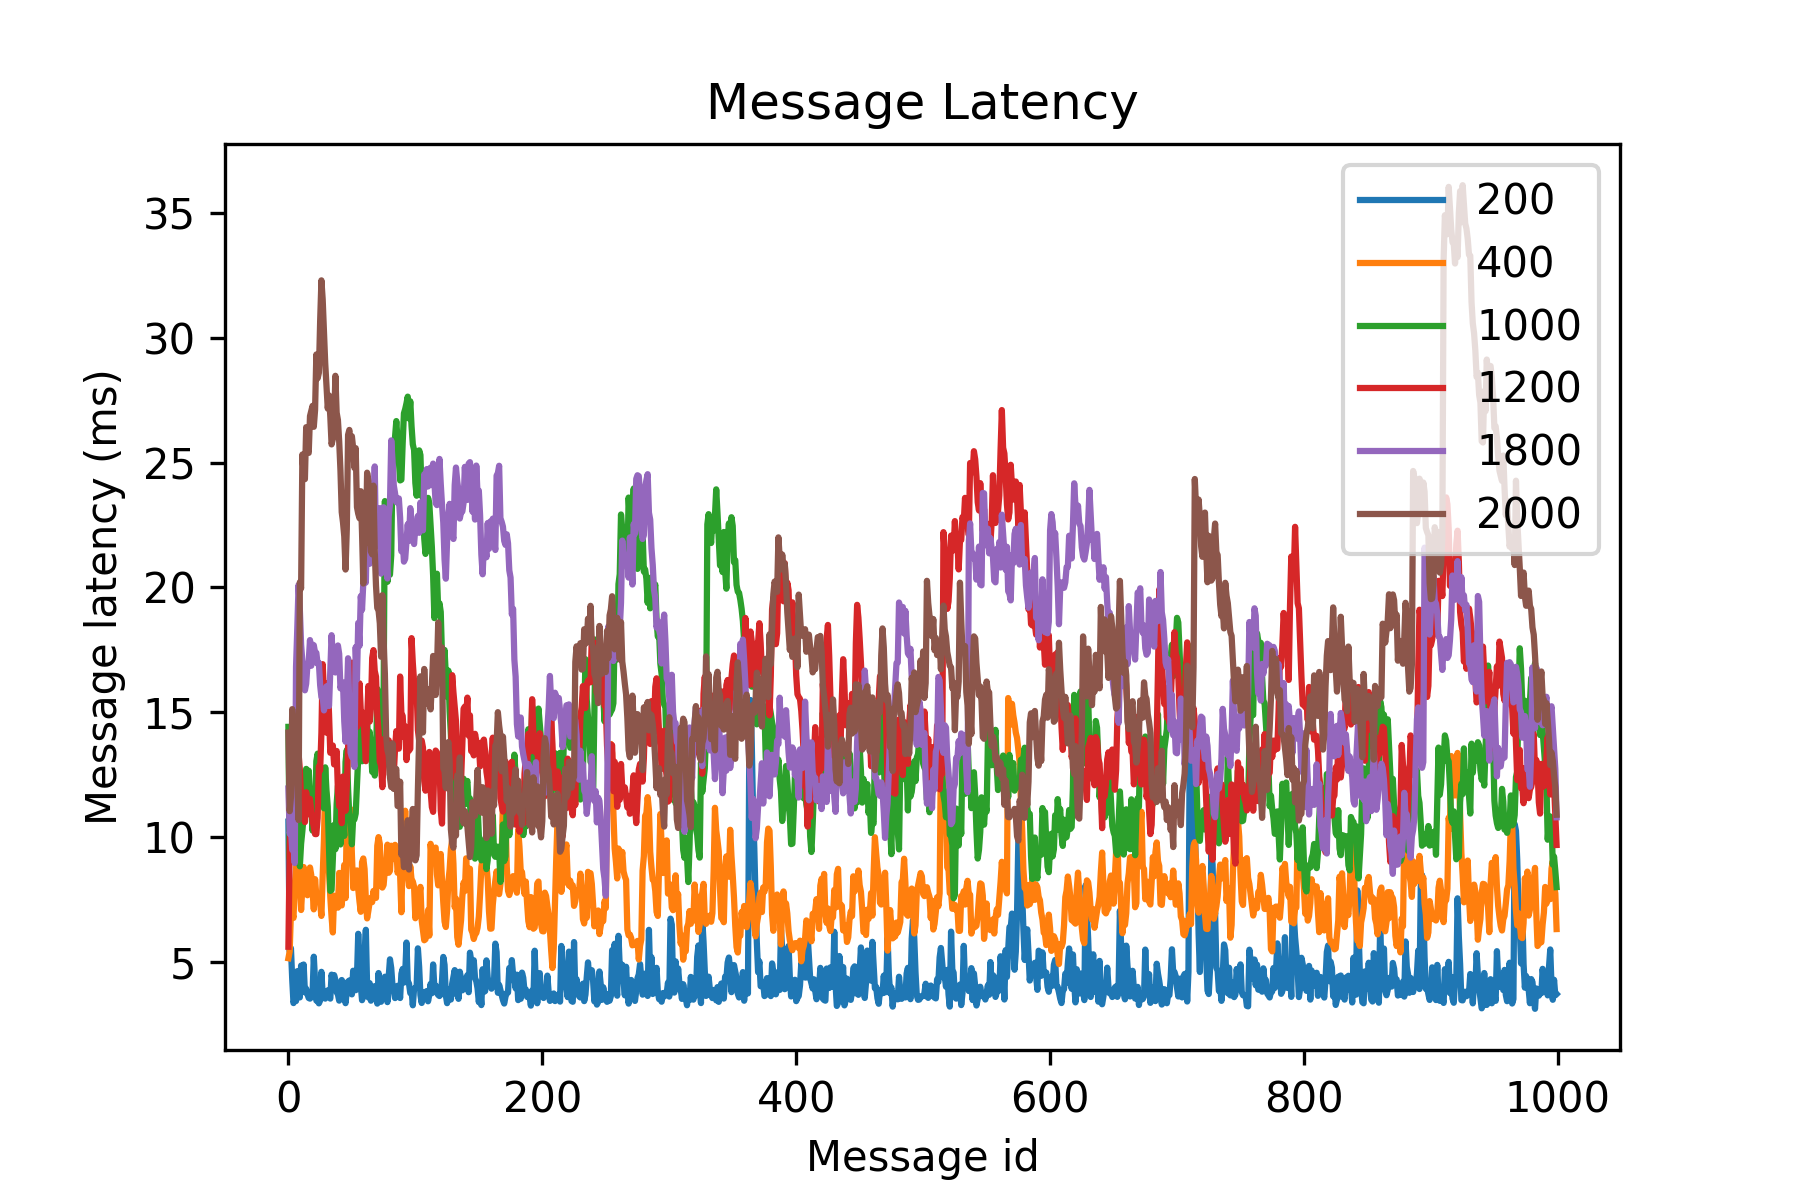
\includegraphics[width = 1\textwidth]{ex1_res2.png}
\caption{Message latency for ROS Melodic on Ubuntu Bionic 64-bit}
\end{figure}

\textbf{Conclusion} \\
1. The message latency from previous experiment by Issac is all almost under 20ms lower latency like 200Hz and 400Hz are very low latency and perform better than higher frequency like 1800Hz and 2000Hz. \\
2. In my experiment, message latency is high and very unstable in ROS kinetic on Ubuntu Xenial 32bits. Message latency can be up to hundreds millisecond which is ten times than previous experiment message latency.\\
3. Then in ROS Melodic on Ubuntu Bionic 64bits, the message latency is low and the result is very like the previous Issac's one. In lower frequency 200Hz and 400Hz show under 10ms latency and in higher message frequency, latency can be vary at 15-20Hz.\\
4. The ROS version and operating system version may have influence on the communication performance between different hosts. Router could also be a factor that have slightly impact on message latency.


\section{Experiment 2: ROS1 and ROS2 message latency comparing}
\textbf{Objective} \\
The aim for this experiment is to compare the message latency in communication between ROS1 and ROS2 in all other same condition. Then have a data analyze for different frequency message to conclude communication performance. 

\textbf{Rationale} \\
In order to acquire a detailed performance characteristics of ROS1 and ROS2 channels, this experiment uses Raspberry Pi 3B+ which installed operating 64-bit ubuntu system. Then communicating by the same router with ROS1 and ROS2 separately. This can guaranteed the same variable and validity of this experiment.

\textbf{Procedure} \\
1. Start one node on one Raspberry Pi and send different frequency message to another host through wifi router. \\
2. Using "rospy" in ROS1 run python2 code which send timestamped messages from the sender host to the echoer host. Then the echoer host send message back to sender host. \\
3. The sender node will receive the message and then record message id and time elapsed in communication into a file.  \\
4. Message frequency is from low frequency (1Hz and 10Hz), middle frequency(100 and 200Hz) and high frequency (1000 and 2000Hz). Every frequency will be run 3 times and get a mean time results.\\
5. Using "rclpy" in ROS2 run python3 code which also send and receive message and then record the results. \\
6. Record all result and plot by using python in Jupyter notebook.

\textbf{Hardware Configuration} \\
4 Raspberry Pi 3B+ \\
TP-Link 150M Router

\textbf{Software Configuration} \\
Ubuntu 18.04 Bionic (64-bit)\\
ROS1 Melodic (Latest, Released May, 2018) \\
ROS2 Crystal Clemmys (Released December 2018)

\textbf{Hypothesis} \\
1. In ROS2 the message latency is lower than ROS1 overall.\\
2. High frequency has lower message latency than lower frequency in both ROS1 and ROS2.

\textbf{Results} \\
Figure 4.4 and 4.5 compare ROS1 an ROS2 message latency from 1Hz to 2000Hz message frequency. Figure 4.6 and Figure 4.7 compare 1Hz and 10Hz message frequency. Figure 4.8 and Figure 4.9 compare 100Hz and 200Hz message frequency. Figure 4.10 and Figure 4.11 compare 1000Hz and 2000Hz message frequency.

\begin{figure}
\begin{minipage}[h]{0.5\linewidth}
\centering
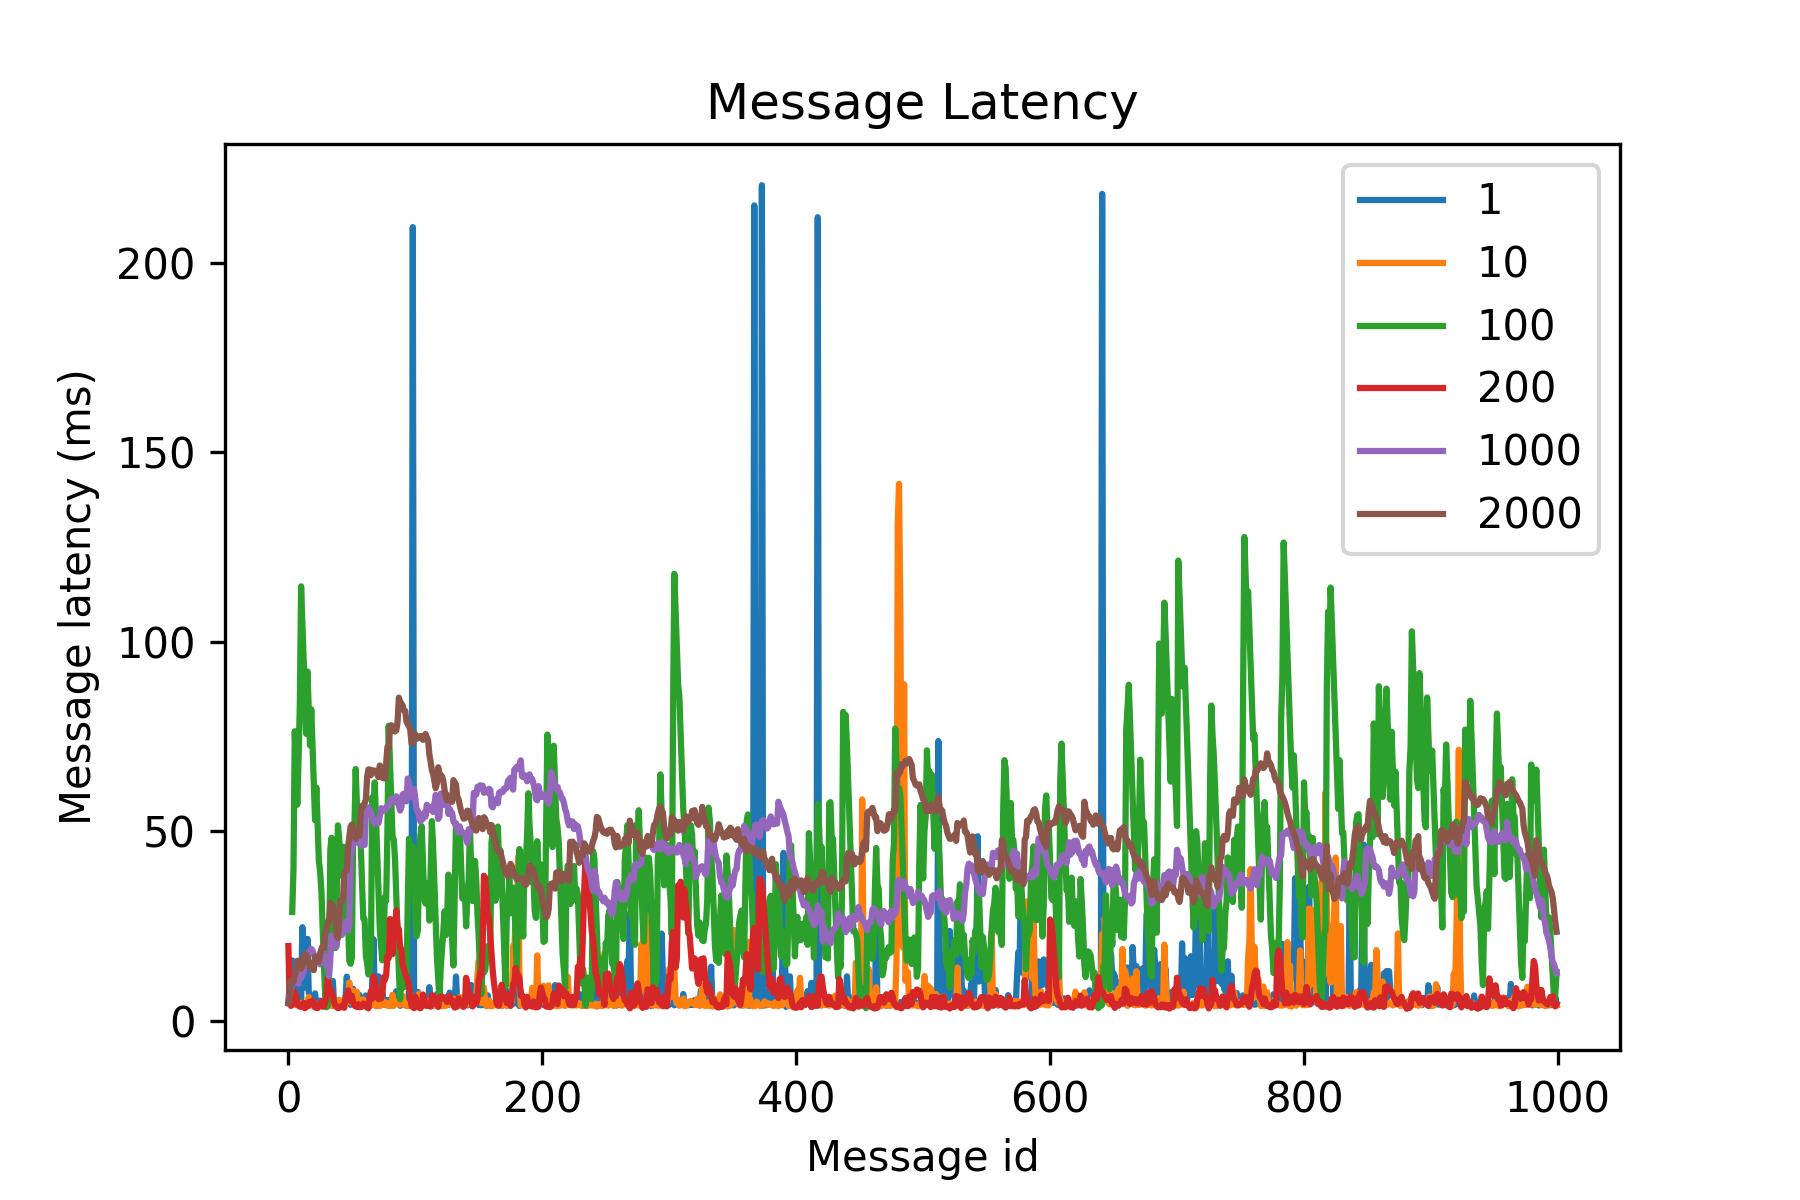
\includegraphics[width = 1\textwidth]{all.png}
\caption{ROS1 all frequency}
\label{fig:side:a}
\end{minipage}%
\begin{minipage}[h]{0.5\linewidth}
\centering
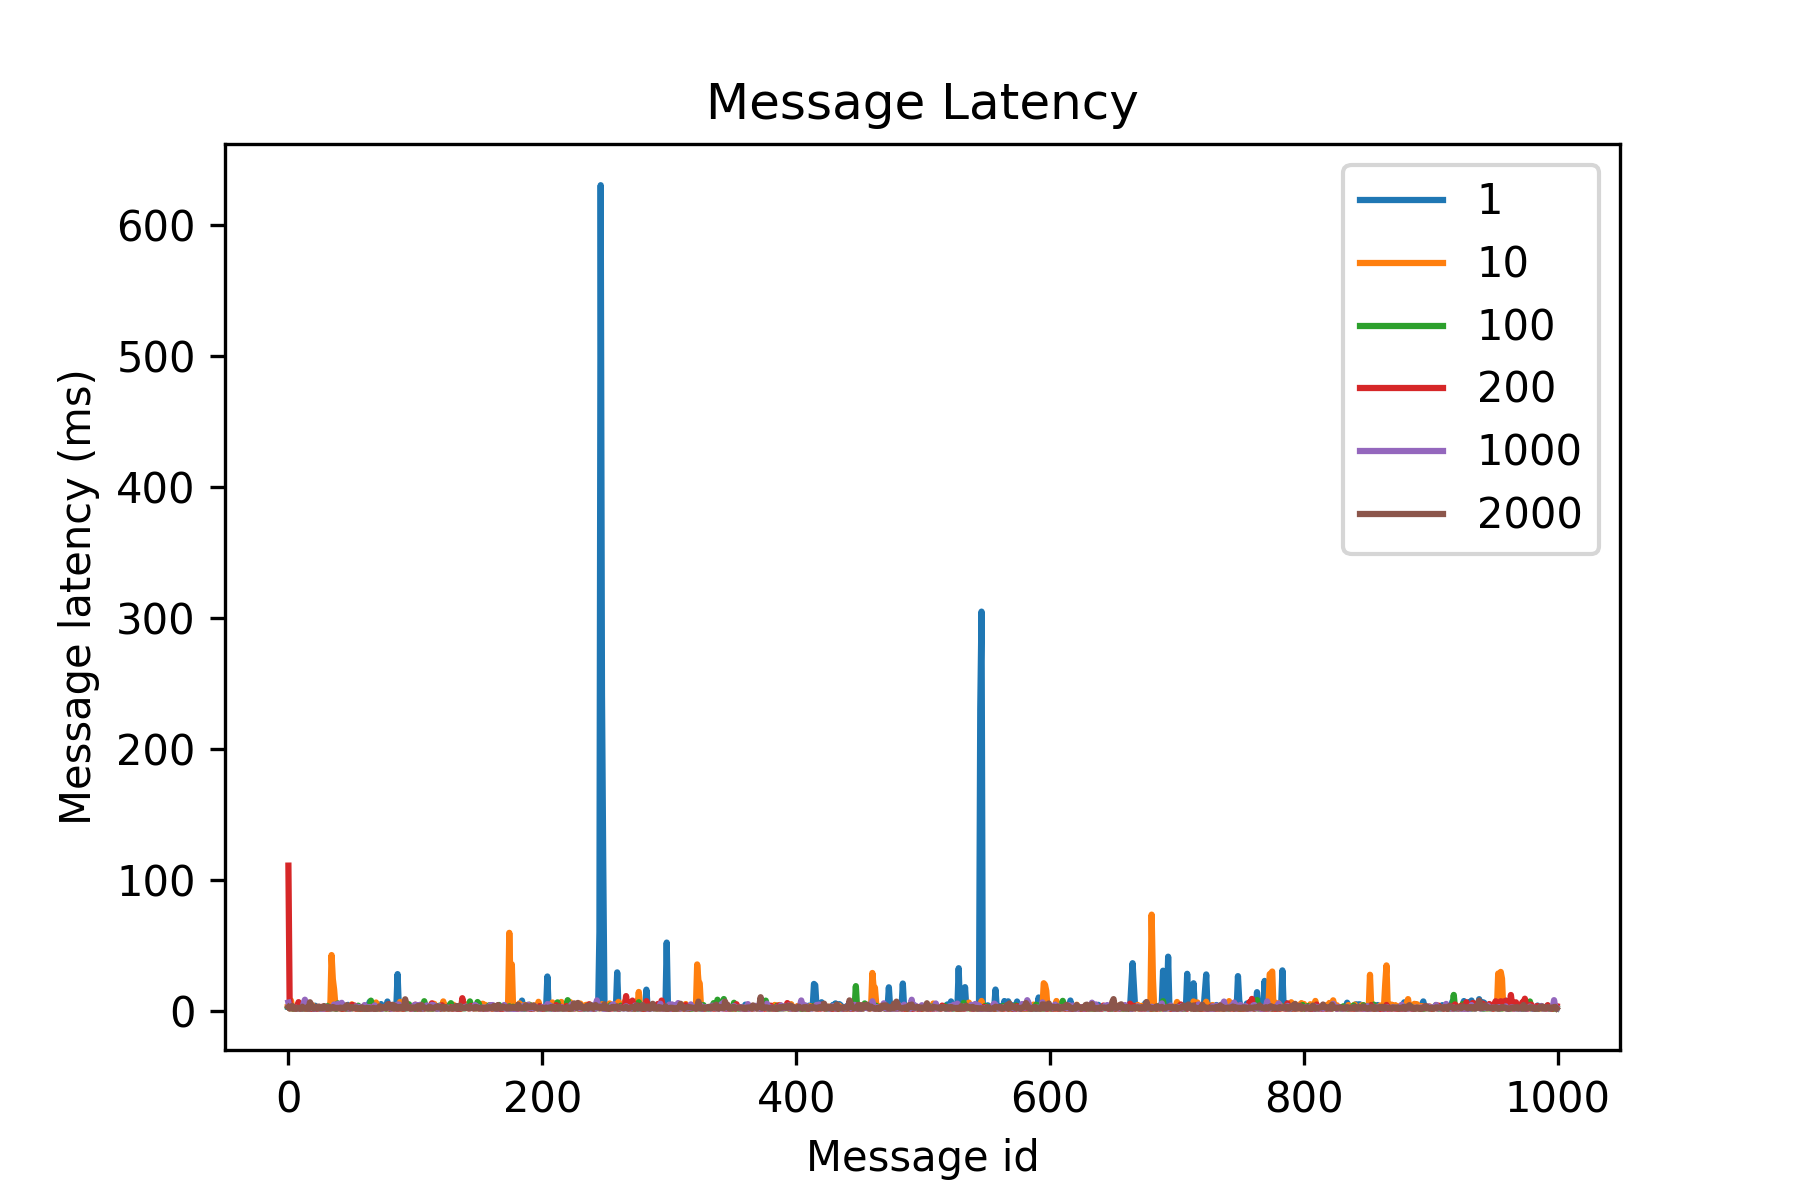
\includegraphics[width = 1\textwidth]{all2.png}
\caption{ROS2 all frequency}
\label{fig:side:b}
\end{minipage}
\end{figure}

\begin{figure}
\begin{minipage}[h]{0.5\linewidth}
\centering
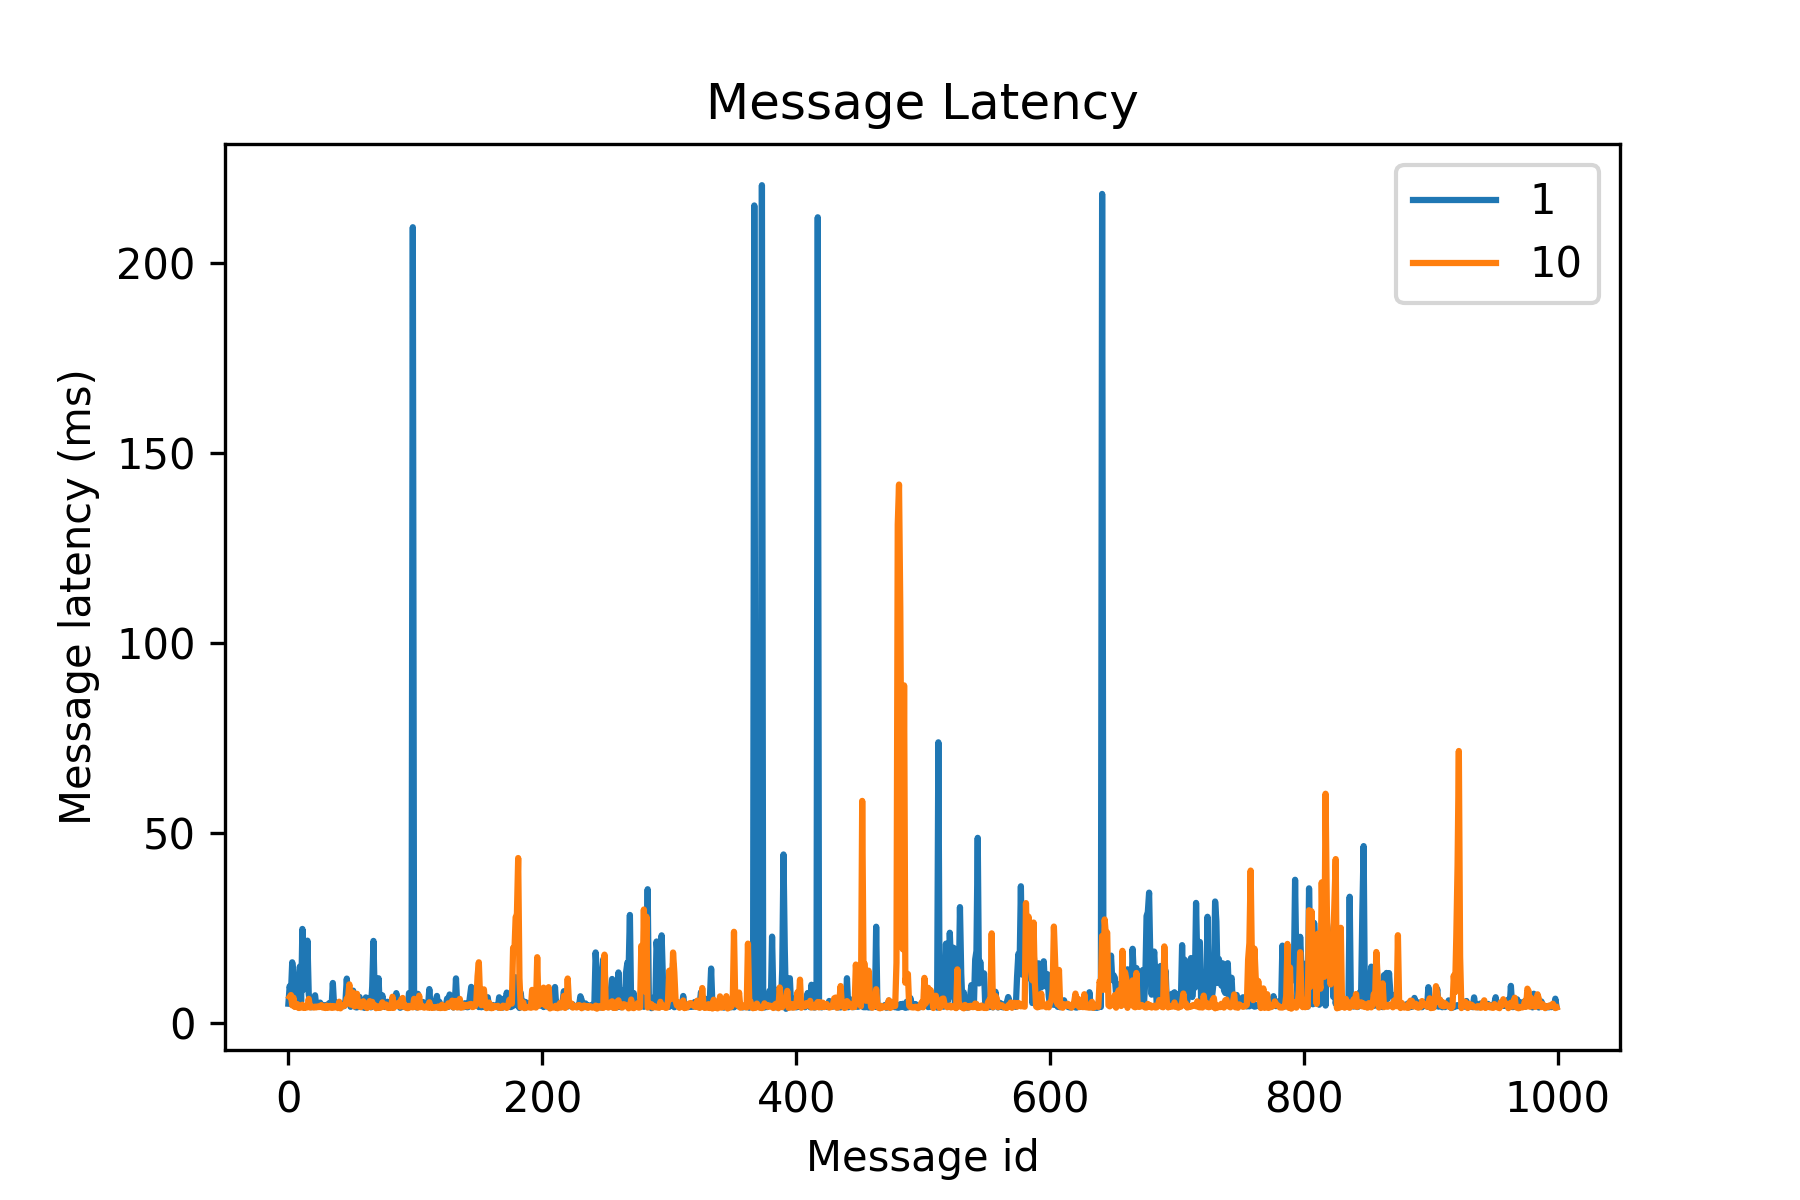
\includegraphics[width = 1\textwidth]{low.png}
\caption{ROS1 1Hz and 10Hz}
\label{fig:side:a}
\end{minipage}%
\begin{minipage}[h]{0.5\linewidth}
\centering
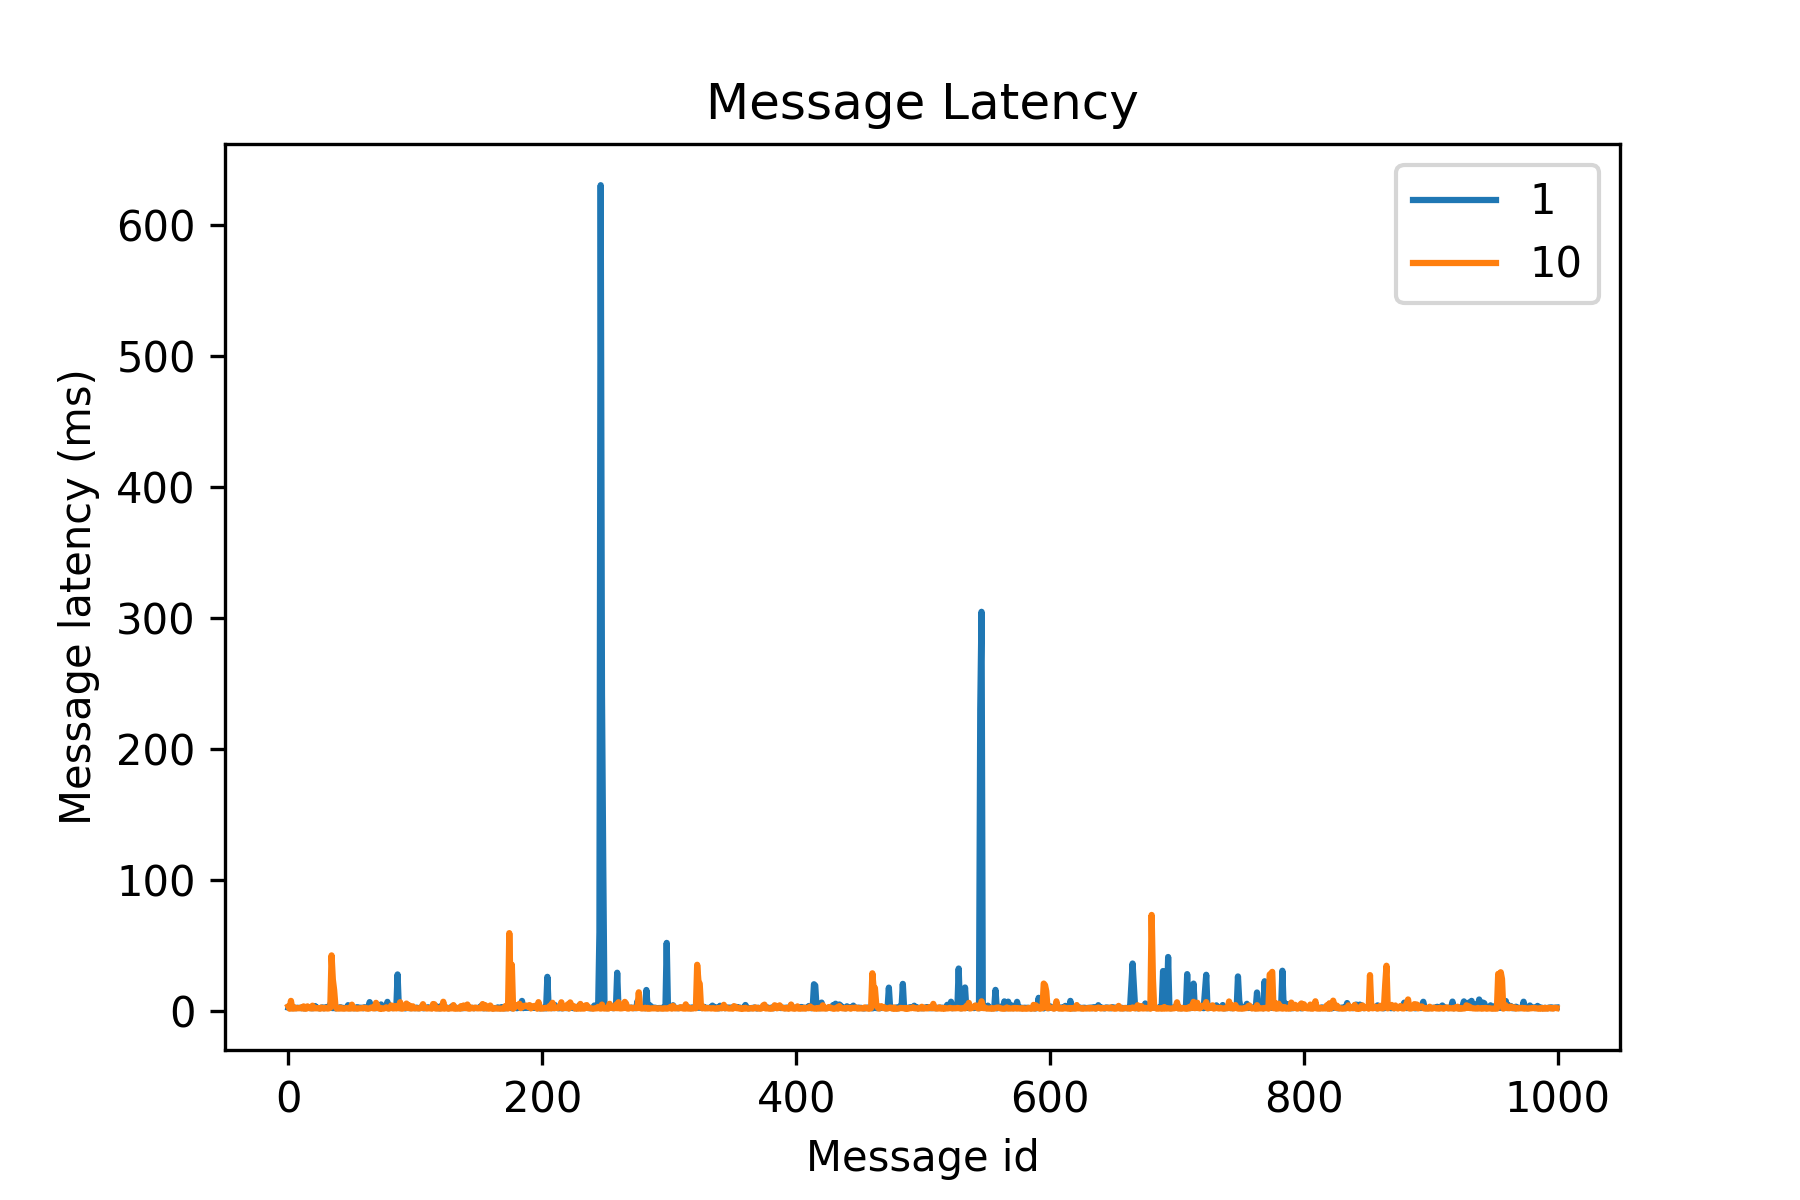
\includegraphics[width = 1\textwidth]{low2.png}
\caption{ROS2 1Hz and 10Hz}
\label{fig:side:b}
\end{minipage}
\end{figure}

\begin{figure}
\begin{minipage}[h]{0.5\linewidth}
\centering
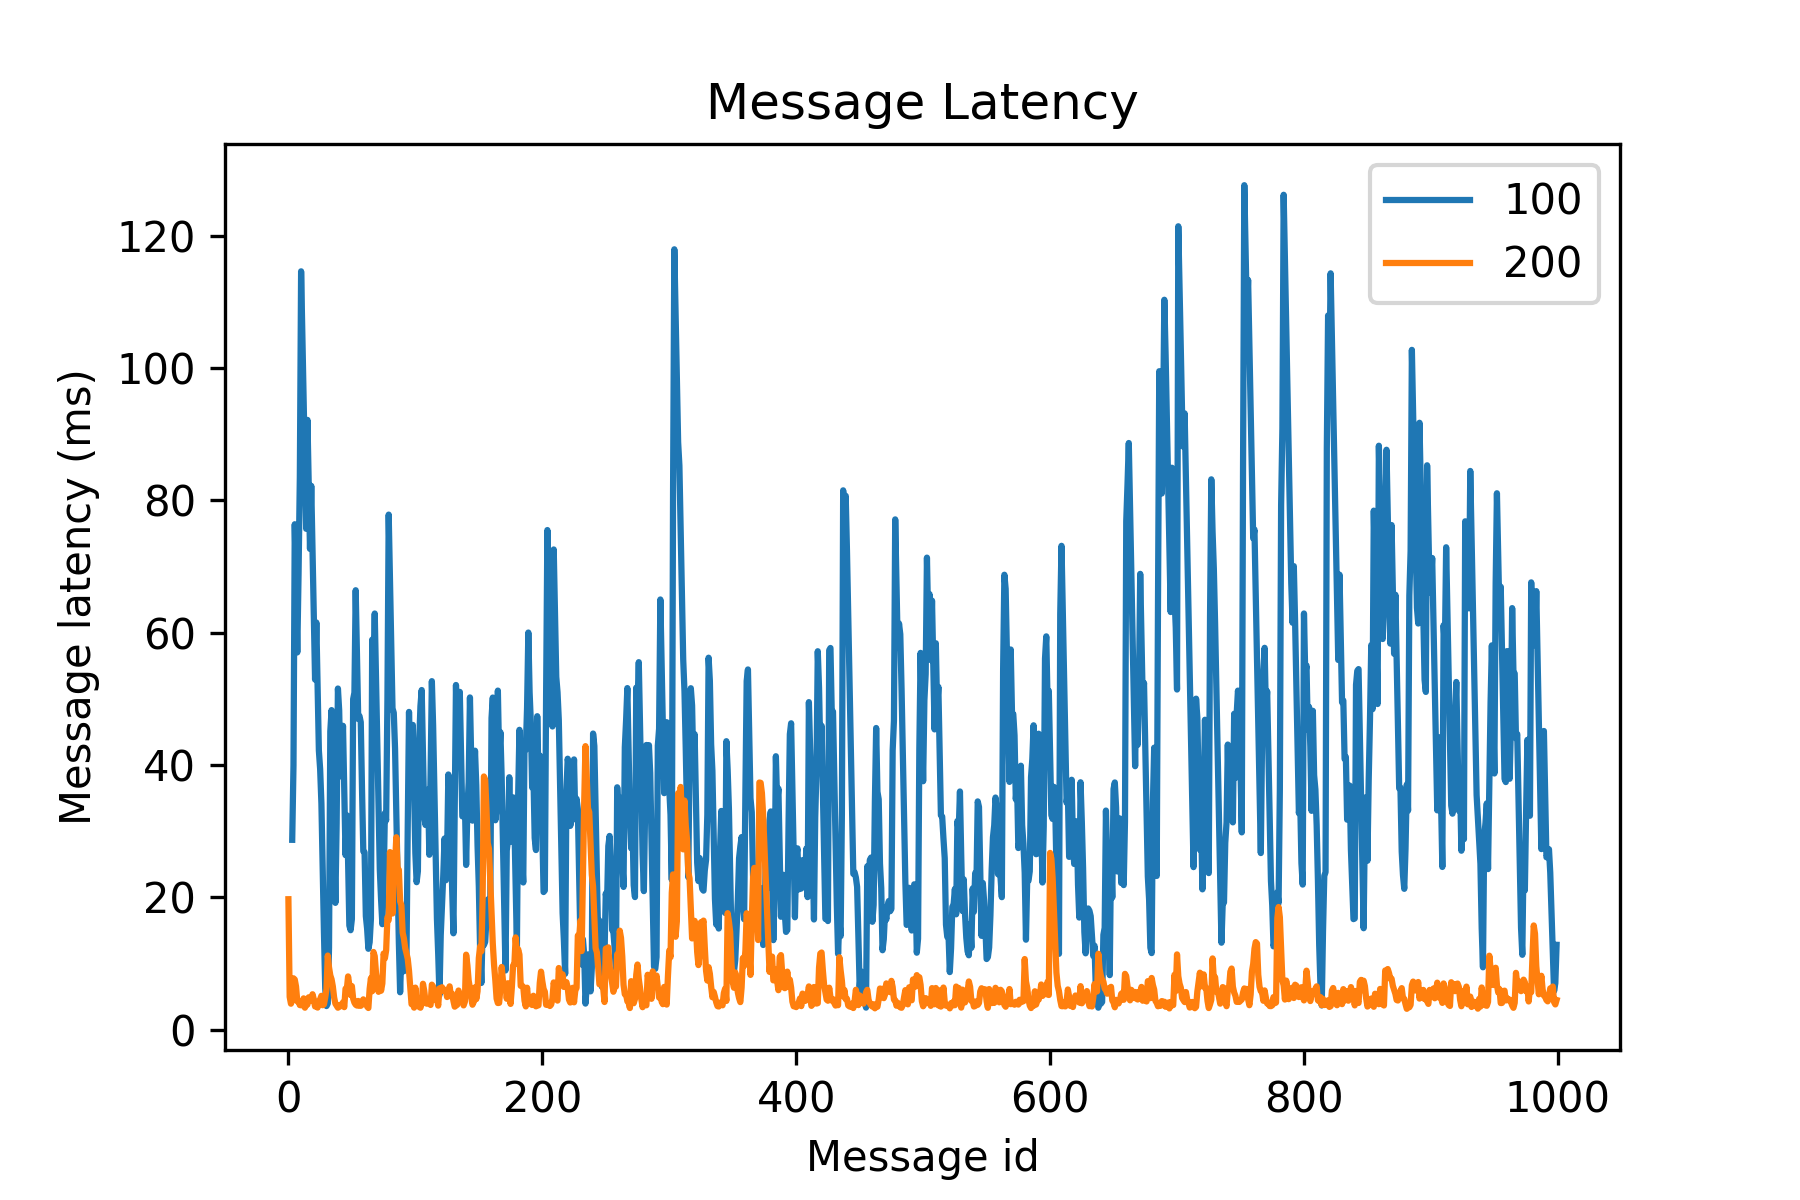
\includegraphics[width = 1\textwidth]{middle.png}
\caption{ROS1 100Hz and 200Hz}
\label{fig:side:a}
\end{minipage}%
\begin{minipage}[h]{0.5\linewidth}
\centering
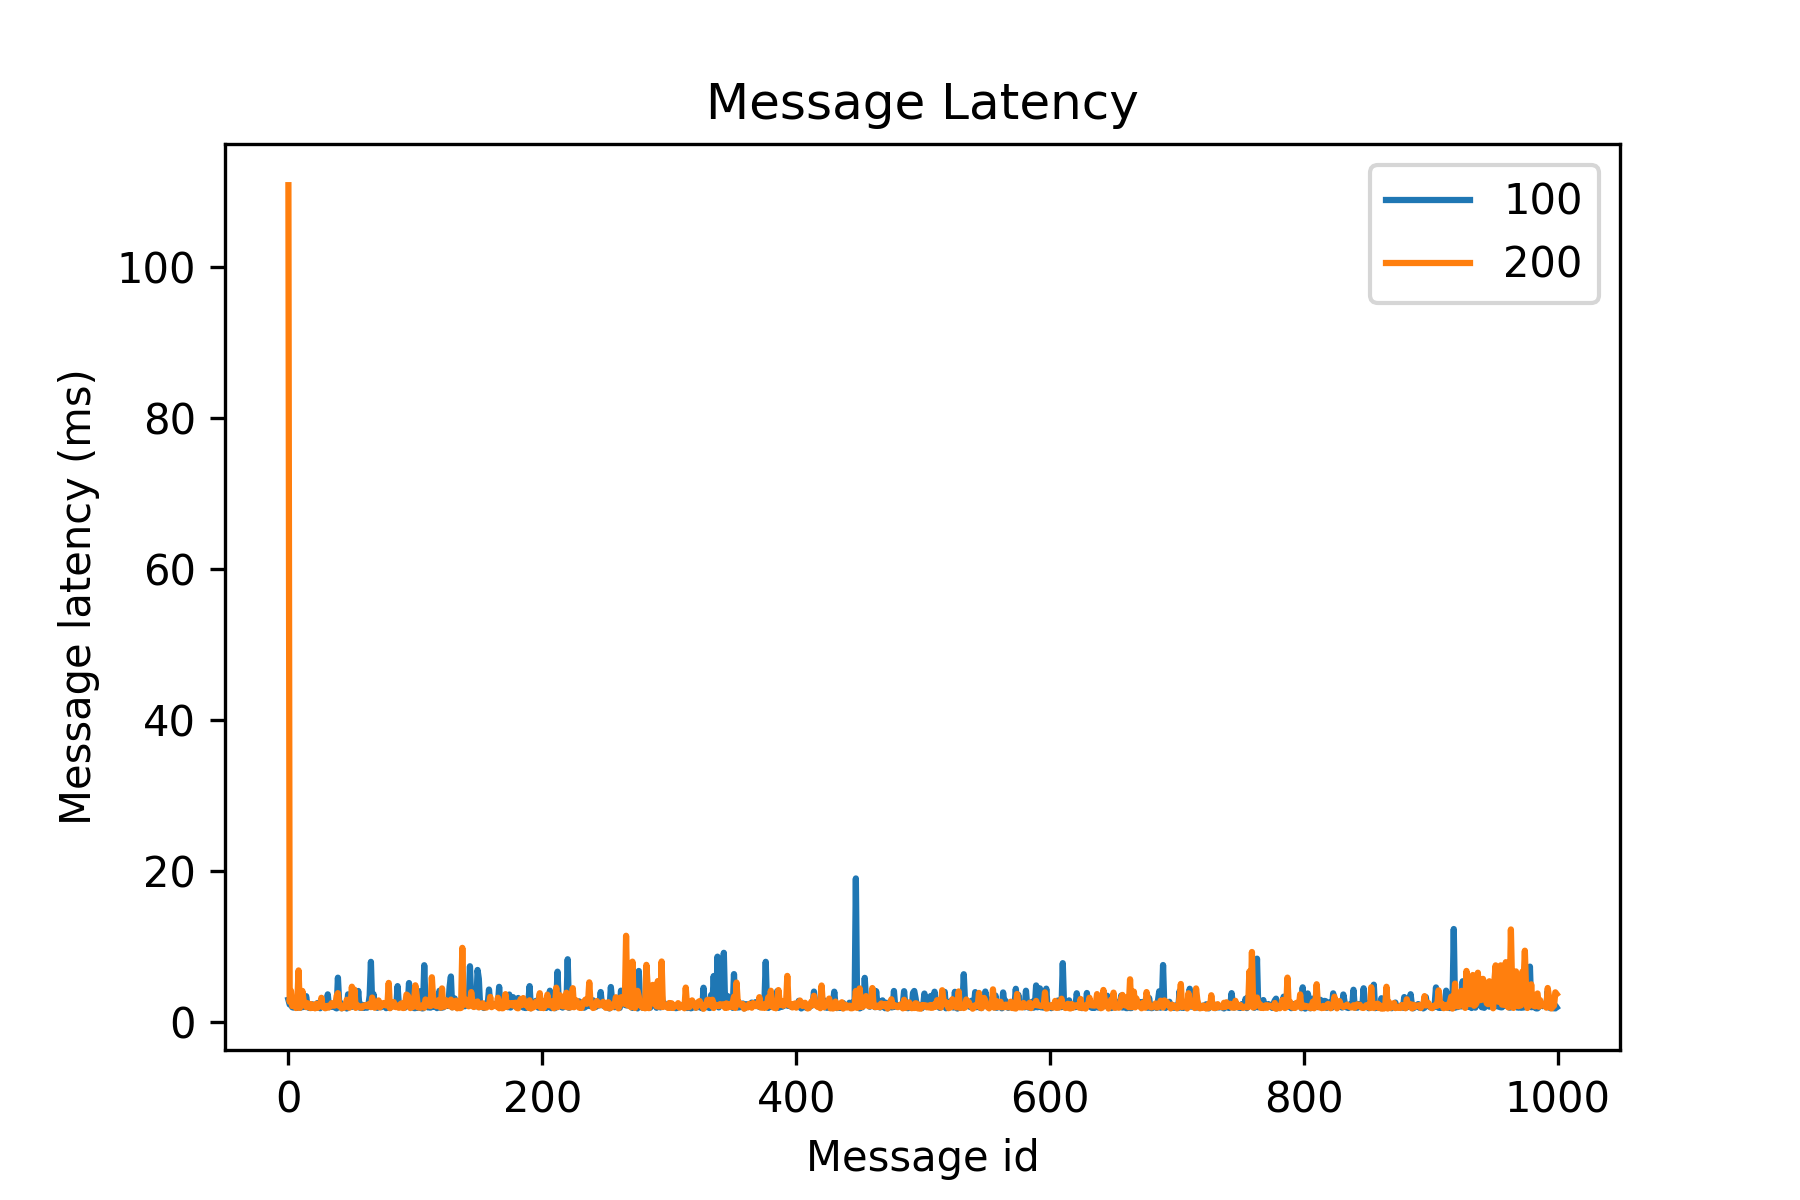
\includegraphics[width = 1\textwidth]{middle1.png}
\caption{ROS2 100Hz and 200Hz}
\label{fig:side:b}
\end{minipage}
\end{figure}

\begin{figure}
\begin{minipage}[h]{0.5\linewidth}
\centering
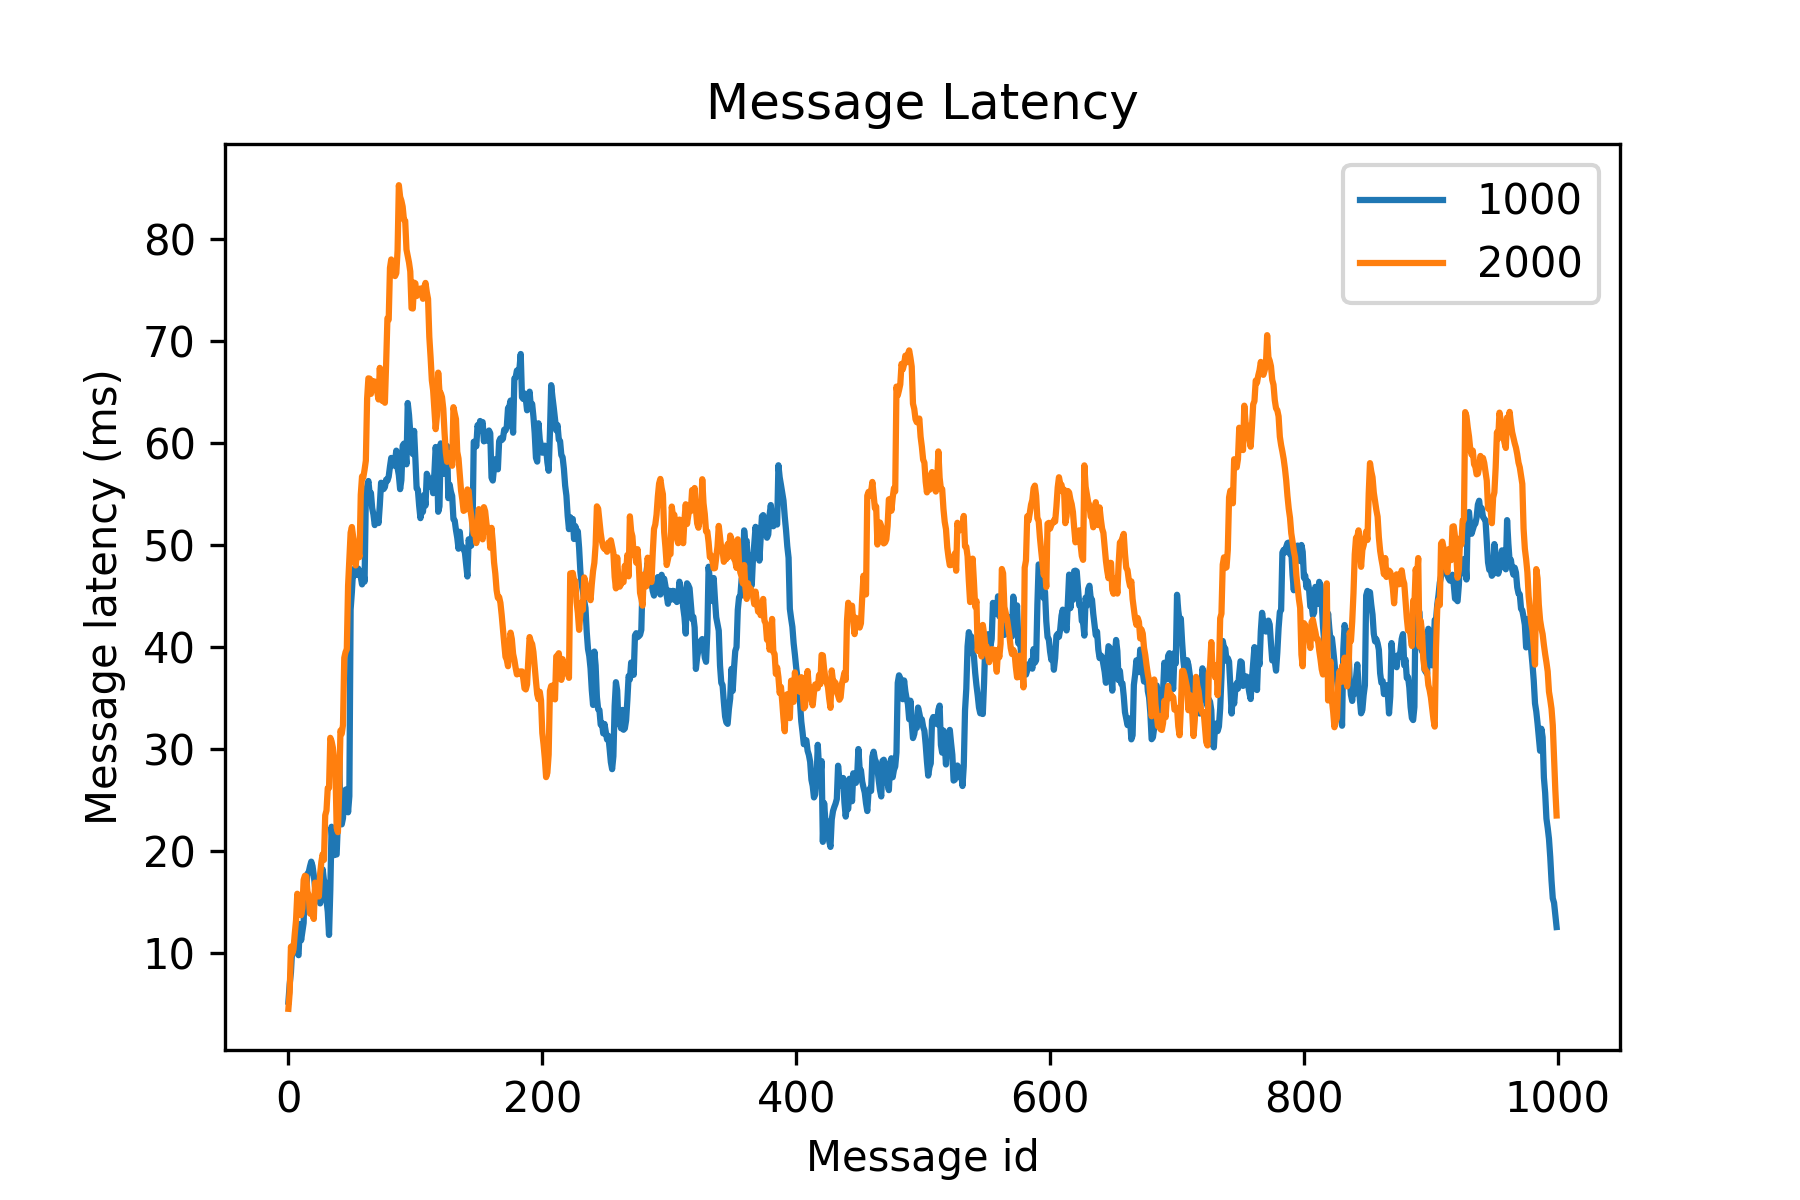
\includegraphics[width = 1\textwidth]{high.png}
\caption{ROS1 1000Hz and 2000Hz}
\label{fig:side:a}
\end{minipage}%
\begin{minipage}[h]{0.5\linewidth}
\centering
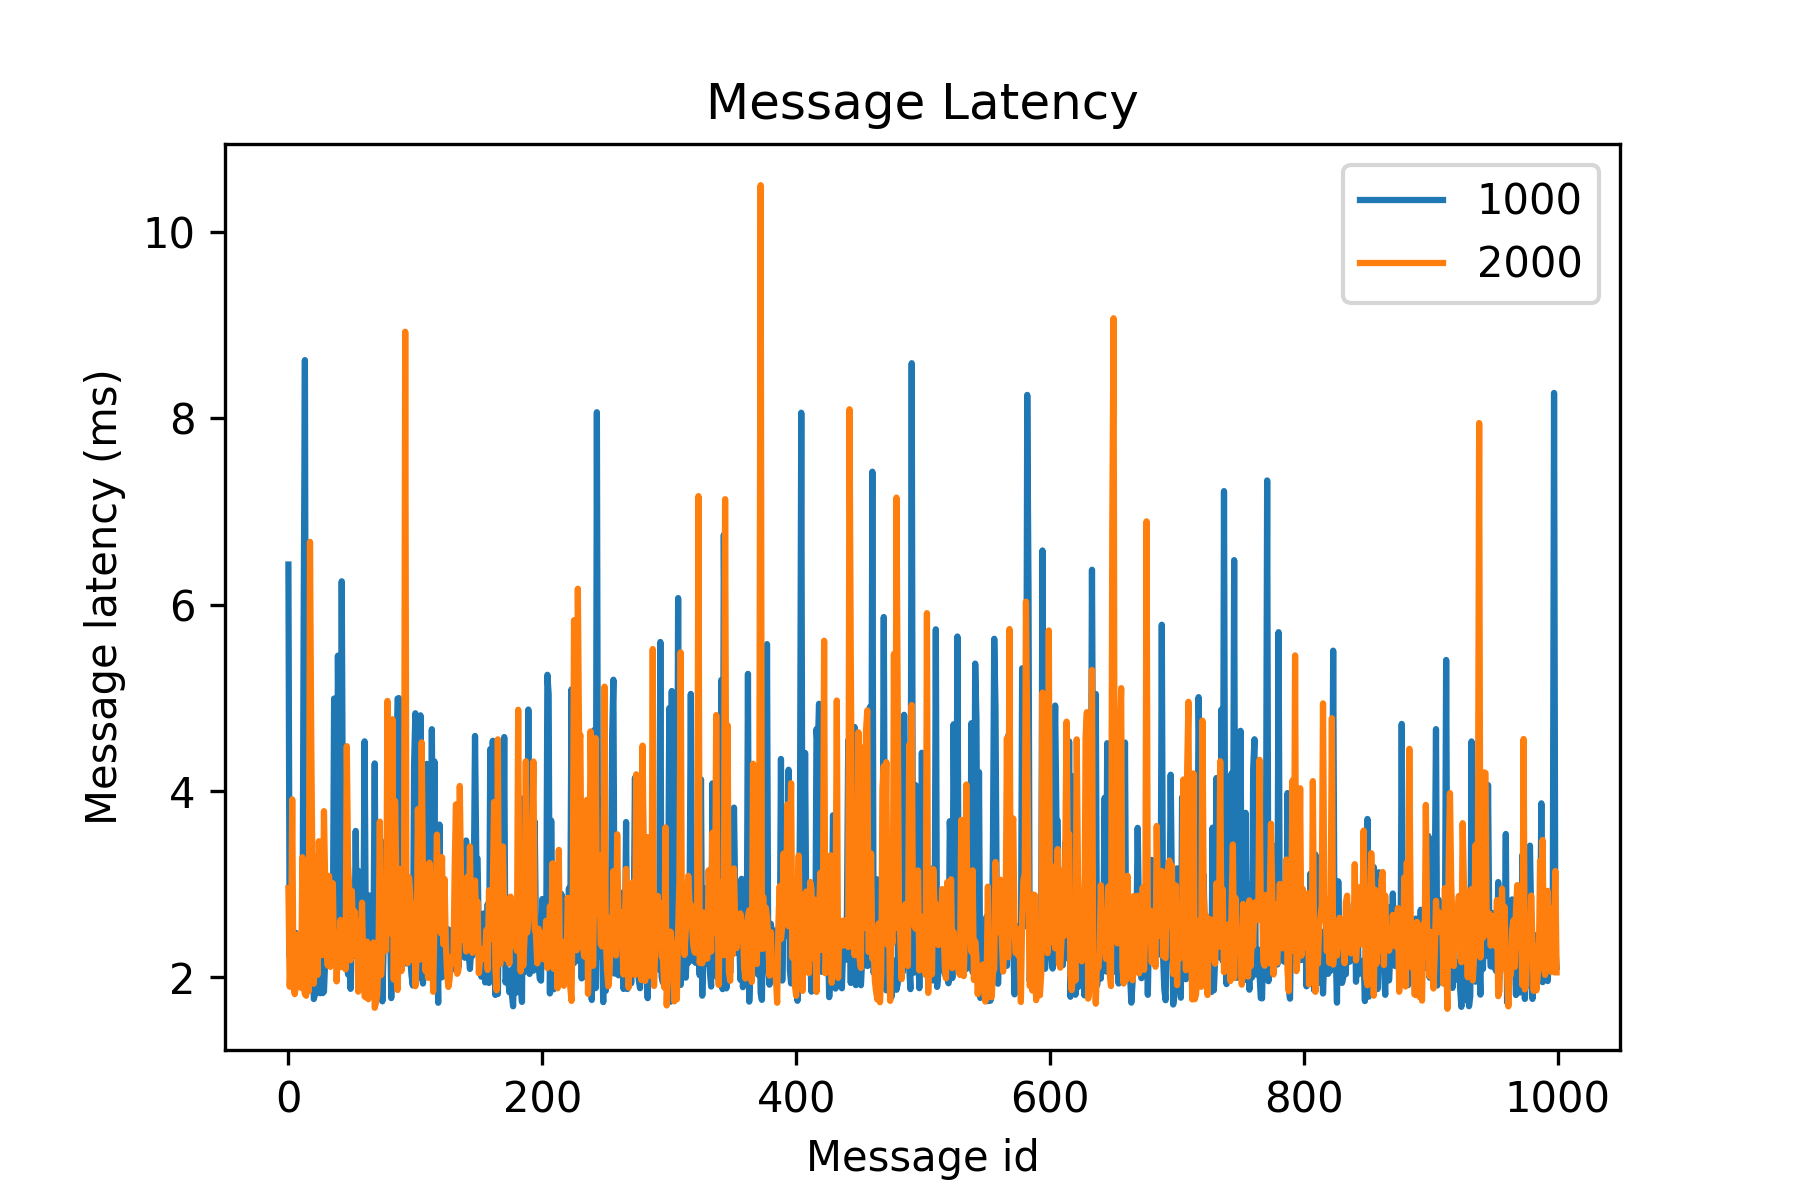
\includegraphics[width = 1\textwidth]{high2.png}
\caption{ROS2 1000Hz and 2000Hz}
\label{fig:side:b}
\end{minipage}
\end{figure}


\textbf{Conclusion} \\
1. From the experiment, overall, ROS1 is less stable than ROS2 from low frequency to high frequency. Most message latency is under 50ms in ROS2, but massage can vary under 100ms in ROS1. \\
2. In low frequency, 1Hz and 10Hz comparing, ROS1 latency is not stable and sometimes shows high frequency over 200ms. However, in ROS2, most message latency is very low, only few message shows high latency that might be the network problem. \\
3. Then in middle frequency, 100Hz and 200Hz message  frequency, ROS1 message latency can vary from 20ms to 100ms. However, ROS2 shows a stable and low message latency under 10ms.\\
4. In High frequency, 1000Hz and 2000Hz, message latency is from 30ms to 70ms in ROS1, which is obviously higher than ROS2 under 10ms.
5. To conclude, ROS2 can show more stable and less message frequency than ROS1 with the same hardware and operating system. Although sometimes there will be network fluctuation causing very high message latency, it may be solved if using better hardware like router.
%%%%%%%%%%%%%%%%%%%%%%%%%%%%%%%%%%%%%%%%%%%%%%%%%%%%%%%%%%%%%%%%%%%
\chapter{Conclusion}\label{conclusion}
\section{Summary}



\clearpage
\section{Future work}



\appendix % first appendix
%%%%%%%%%%%%%%%%%%%%%%%%%%%%%%%%%%%%%%%%%%%%%%%%%%%%%%%%%%%%%%%%%%%
\chapter{First appendix}

\section{ROS1 installation commond steps}

\begin{verbatim}
# Install system

sudo sh -c 'echo "deb http://packages.ros.org/ros/ubuntu $(lsb_release -sc)
main" > /etc/apt/sources.list.d/ros-latest.list'
sudo apt-key adv --keyserver 'hkp://keyserver.ubuntu.com:80' --recv-key
C1CF6E31E6BADE8868B172B4F42ED6FBAB17C654
sudo apt update
sudo apt install ros-melodic-ros-base

# Install tools and dependencies

sudo rosdep init
rosdep update
echo "source /opt/ros/melodic/setup.bash" >> ~/.bashrc
source ~/.bashrc
sudo apt install python-rosinstall python-rosinstall-generator python-wstool 
build-essential

# Start ROS service and create workspace

roscore
create catkin folder
mkdir -p ~/catkin_ws/src
cd ~/catkin_ws/
catkin_make
source devel/setup.bash

\end{verbatim}

\section{ROS2 installation steps}

\begin{verbatim}
# Install 
sudo locale-gen en_US en_US.UTF-8
sudo update-locale LC_ALL=en_US.UTF-8 LANG=en_US.UTF-8
export LANG=en_US.UTF-8
sudo apt update && sudo apt install curl gnupg2 lsb-release
curl -s 
https://raw.githubusercontent.com/ros/rosdistro/master/ros.asc | sudo apt-key add -
install
export CHOOSE_ROS_DISTRO=crystal
sudo apt update
sudo apt install ros-$CHOOSE_ROS_DISTRO-ros-base

# Environment setup
sudo apt install python3-argcomplete
source /opt/ros/$CHOOSE_ROS_DISTRO/setup.bash
echo "source /opt/ros/$CHOOSE_ROS_DISTRO/setup.bash" >> ~/.bashrc
sudo apt install python3-colcon-common-extensions

# create workspace
mkdir -p ~/ros2_example_ws/src
cd ~/ros2_example_ws

\end{verbatim}
\textit{/etc/hosts}
\begin{verbatim}
ff02::1 ip6-allnodes
ff02::2 ip6-allrouters

192.168.1.11 com1
192.168.1.12 com2
\end{verbatim}
\textit{config.sh}
\begin{verbatim}
# /bin/sh
export ROS_HOSTNAME=com1
export ROS_IP=192.168.1.11
export ROS_MASTER_URI=http://com1:11311/
\end{verbatim}

%%%%%%%%%%%%%%%%%%%%%%%%%%%%%%%%%%%%%%%%%%%%%%%%%%%%%%%%%%%%%%%%%%%
\chapter{Second appendix}

%%%%%%%%%%%%%%%%%%%%%%%%%%%%%%%%%%%%%%%%%%%%%%%%%%%%%%%%%%%%%%%%%%%
% it is fine to change the bibliography style if you want
\bibliographystyle{plain}
\bibliography{mproj}
[1] Sandra May. What Is Robotics?  \url{https://www.nasa.gov/audience/forstudents/k-4/stories/nasa-knows/what_is_robotics_k4.html}. Nov. 9, 2009

[2] B. Bauml and G. Hirzinger. Agile Robot Development (aRD): A Pragmatic Approach to Robotic Software. In 2006 IEEE/RSJ International Conference on Intelligent Robots and Systems, pages 3741–3748, Oct 2006.

[3] Avinash Gautam and Sudeept Mohan. A review of research in multi-robot systems. In 2012 IEEE 7th International Conference on Industrial and Information Systems (ICIIS), pages 1–5. IEEE, Aug 2012.

[4] Pedro U. Lima and Luis M. Cust´odio. Multi-Robot Systems. In Innovations in Robot Mobility and Control, pages 1–64. Springer, Berlin, Heidelberg, Aug 2005.

[5] Zhi Yan, Nicolas Jouandeau, and Arab Ali Cherif. International Journal of Advanced Robotic Systems, 10(12):399, 2013.

[6] Deborah Estrin, David Culler, Kris Pister, and Gaurav Sukhatme. Connecting the physical world with pervasive networks. IEEE pervasive computing, 1(1):62–63, 2002.

[7] Cellan-Jones. A£15 computer to inspire young programmers. BBC news. 5 May 2011

[8] Gibbs, Samuel. Raspberry Pi becomes best selling British computer. The Guardian. Retrieved 28 December 2016.

[9] SunFounder PiCar-S Kit V2.0 page. \url{https://www.sunfounder.com/picar-s-kit.html}. 

[10] Isaac Jordan. Robotic Middleware. \url{https://github.com/Sheepzez/ros-multirobot-evaluation/tree/master/experiments/message_latency/no_ echo_delay_no_disk_write}. 2017-03-18.

[11] ROS Melodic Morenia. \url{wiki.ros.org}. Retrieved 10 June 2018.

[12] The Robotics Back-End Home page. \url{https://roboticsbackend.com/what-is-ros}. 2019

[13] ROS2 Overview Home page. \url{https://index.ros.org/doc/ros2/}

[14]  Brian Gerkey. Why ROS 2?. \url{http://design.ros2.org/articles/why_ros2.html}

[15]"Ubuntu and Debian". Ubuntu.com. Canonical Ltd. Retrieved 14 December 2013.

[16]"Ubuntu and Debian". Ubuntu.com. Canonical Ltd. Retrieved 14 December 2013.

[17] What is Ubuntu MATE?. Ubuntu MATE Team. \url{https://ubuntu-mate.org/what-is-ubuntu-mate/}. 2019 

[18] Star topology. \url{http://www.telecomabc.com/s/star.html}. 2015

[19] Star topology. Cisco Networking Academy 2014.

[20] Topics. \url{http://wiki.ros.org/Topics}. 2019-02-20

[21] TCPROS. \url{http://wiki.ros.org/ROS/TCPROS}. 2013-04-15 

[22] ROS on DSS. \url{https://design.ros2.org/articles/ros_on_dds.html}

[23] Why Consider DDS. ROS on DSS. \url{https://design.ros2.org/articles/ros_on_dds.html}

[24] Where did DDS come from. ROS on DSS. \url{https://design.ros2.org/articles/ros_on_dds.html}

[25] Issac Jordan. Experiment \url{https://github.com/Sheepzez/ ros-multirobot-evaluation/tree/master/experiments/message_latency/ bag-sender-receiver}. Accessed: 2017-03-18.

[26] Drone (UAV) \url{https://internetofthingsagenda.techtarget.com/definition/drone}. July 2019

[27] Sunfounder Smart Video Car Kit for Raspberry Pi. \url{https://github.com/sunfounder/Sunfounder_Smart_Video_Car_Kit_for_RaspberryPi}.

[28] ROS 2 Overview. \url{https://index.ros.org/doc/ros2/}.


\end{document}
